\documentclass[12pt]{article}
\usepackage{graphicx}
\usepackage{caption}
\usepackage{subcaption}
\usepackage{verbatim}
\usepackage{url}
\usepackage{listings}
\usepackage{epsfig}
\usepackage[margin=3cm]{geometry}
%\usepackage{titling}
%\setlength{\droptitle}{-12em}

%% Define a new 'leo' style for the package that will use a smaller font.
\makeatletter
\def\url@leostyle{%
\@ifundefined{selectfont}{\def\UrlFont{\sf}}{\def\UrlFont{\small\ttfamily}}}
\makeatother
%% Now actually use the newly defined style.
\urlstyle{leo}

\title{ Private Dropbox \\ Final Report \\ COSC480}
\author{Calum O'Hare \\ Supervisor: David Eyers}
\date{}

\begin{document}
\maketitle

\begin{comment}
\null
\vfill
\end{comment}
\newpage
%\section*{Abstract}
\begin{abstract}
Private Dropbox is a file synchronisation tool designed to
keep files in sync across multiple devices. It is decentralised,
unlike many other file hosting services like Dropbox.
My program is designed to run across any given network
of computers. Configuration files allow
the user to specify what files should be synchronised; to which
machines; and how often to sync them. My program monitors the 
files being synchronised and the last time files
were updated so that it knows when to sync with any
other connected machines. Different machines may require different replication
strategies, this makes it unique from other file replication tools.
%I have written a program in Python which reads user
%settings from a file, and synchronises the appropriate files
%to the appropriate machines when they have been modified.
%It does this using an efficient two-way file synchronising tool called
%Unison. I will discuss in this dissertation what I have done and
%how I have tested my program.
\end{abstract}
\newpage

\tableofcontents
\newpage

\section{Introduction}
Dropbox is a well known online file hosting tool that will
keep your data synchronised across multiple devices. I feel
that there is a need for a private file synchronisation tool
controlled by the end user rather than a corporation. In this
section I will outline my project goals which explain how
my program differs from Dropbox and others; give background
information about the alternatives like Dropbox and what the
problems with these solutions are; outline an example
use case which shows why my program will be useful.

\subsection{Project goals}
The aim of this project was to develop a file synchronisation tool.
Similar to  Dropbox (and others) its main function should be to
keep data synchronised between multiple devices.
What makes it different however is it should:
\begin{itemize}
\item Support decentralised operation. It will not necessarily need to communicate with
`the cloud'. The program should not require a
%``the cloud''
centralised server. However it should be
possible to configure the system to behave like a centralised system if the user wants to.
The system should be flexible in this regard.

\item Allow file synchronisation between multiple clients not just point-to-point
between two clients. Synchronisation between two clients however is the
basis for multiple client synchronisation. Clients may be
running different operating systems. Clients may be connected to
different networks, with different costs of access, including being disconnected
from the Internet at times.

\item Permit the user to choose what to replicate and how often to do
it within different sets of files. Choosing what to replicate could be done
based on file name, file types, file size \emph{etc}. They system should
allow for fine-grained user control for the majority of the program's functionality.
\begin{comment}
\item Allow for fine-grained user control for the majority of the program's
functionality, \emph{e.g.}, how often, and what, to replicate within different sets of files. 'What' could be file name, file type, file size, \emph{etc}.
\end{comment}

\item Show statistics about which files are being replicated, their efficiency (time
taken for the files to become fully up to date),
and cost (bandwidth, disk space used). These statistics could also possibly lead
to a heuristic for when to synchronise a given file. For example if a file is
updated and a node has many neighbours to potentially send the file to. Perhaps
choosing the neighbour whose links has the lowest cost would be a good choice
to send the data to first.

\item Operate automatically, without the user having to initiate a file
synchronisation themselves. 
The system's autonomous operation should be influenced by the users
choices on how often to sync and what files should be synced, this
relates to the fine-grained controls mentioned above.
%The user should be able to set when and
%where they would like synchronisation to occur.
\end{itemize}
\subsection{Background}
There are already many services available
that can synchronize your files between different devices. 
Dropbox, Google Drive, Microsoft SkyDrive, Apple iCloud
are all examples of cloud-based solutions for distributing
your files across your devices. The problems with these
services is privacy and availability. Storing your data with a
third party gives them access to your documents. If you
are a commercial organisation with sensitive information
this might be concerning. You could
of course choose to encrypt your files. Encrypting your files adds
two slow extra steps, encrypting them before you upload and decrypting
files before you can use them. This is less than ideal. 
You also cannot guarantee
that you will always be able to access your data, if
the company that hosts your data goes bankrupt or
decides to shutdown their service
you could lose all
of your data with little or no warning. 
For example Megaupload, a file hosting service,
has recently been shut down by the United States Department of
Justice for alleged copyright infringement. According to
its founder, 100 million users lost access to 12 billion
%unique files\cite{dotcom-trial}.
unique files\footnote{http://computerworld.co.nz/news.nsf/news/kim-dotcom-wants-his-money-back}.

There are other possible approaches to replicating files
across multiple computers. For example you could use
version control systems like Subversion and
CVS. One problem with these is that they are
centralised (they rely on a central server); should that
server fail the replication will break. Not only
that, they create a bottleneck at the server which can slow
replication down.
Cloud-based solutions are often centralised. 
Another problem is that even if they are decentralised
like Git or Mercurial, they will not automatically push updates to other
working sets. This could be accomplished with some
Cron scripts or a post-commit hook to get Git to
propagate data onwards. Git might have made a promising
base to build my application on top of; the only real
problem was the version control overhead that comes with
it. Old revisions would take up space on the hard disk
and require more data to be transmitted across network links.
I decided that as a file synchronisation program, revision
history was out of scope and that my program would
deal with just keeping files in sync. Using Git would be
an interesting extension to my program and could easily
be integrated into my current system.

%How about Git? It is a distributed tool.
%Auto push updates to other working sets can be done with a few crond scripts

%Add more here?

%\subsection*{Example use case}
\subsection{Example use case}
Here is an example use case demonstrating why I find my program useful.

I like to keep all of the data on my laptop backed up to an
external hard drive. The data on my computer that I wish
to back up falls into three main categories: documents, music, and movies.
Documents are mostly scripts and programs that I am writing for
University or work projects. Documents also include reports for
assessment. These documents change very frequently and are very important
to me. Often these are small files (but not always). My music collection
changes relatively infrequently, files are $\approx$5MB and I like to
have a relatively current backup of this collection. My movie collection
contains fairly large files but I do not need it to be backed up very often
as it does not change very much and I do not care if I loose some of these
movies. Files that I work on at University would be very useful to have
on my laptop at home. Files that I work on at work mostly stay at work
but occasionally I might want to bring something home to work on.
The other device I always have with me and may be on one of any given
(Wi-Fi or 3G) network at a certain time is my smart phone. I would like
to have photos taken on this backed up to either (or both) my laptop and
external hard drive. 

Some of the files that I move around are of a sensitive or personal nature
and I would prefer not to store them with a third party vendor.
I also have different synchronisation requirements for different
types of data. 
For example my collection of large video files does not change that often
and will chew up valuable network bandwidth whenever it has to transfer
a new file. I like this to be replicated only occasionally as I do not
use it that much. On the other hand my document collection which I use
for work and coursework changes very often, is very important, and
is fairly small. I would like this to be as up to date as possible.

Existing file synchronisation tools do not do enough
for me. I do not have enough control over my data.
I want to know which machines my files are going to and when.
I want to feel confident that I will always be able to access
my data even if the service closes down or my internet connection
fails. My program is aimed at addressing these issues.

%Look at this it is repetitive of above section

\begin{figure}[htp]
    \begin{subfigure}[b]{1\textwidth}
        \centering
        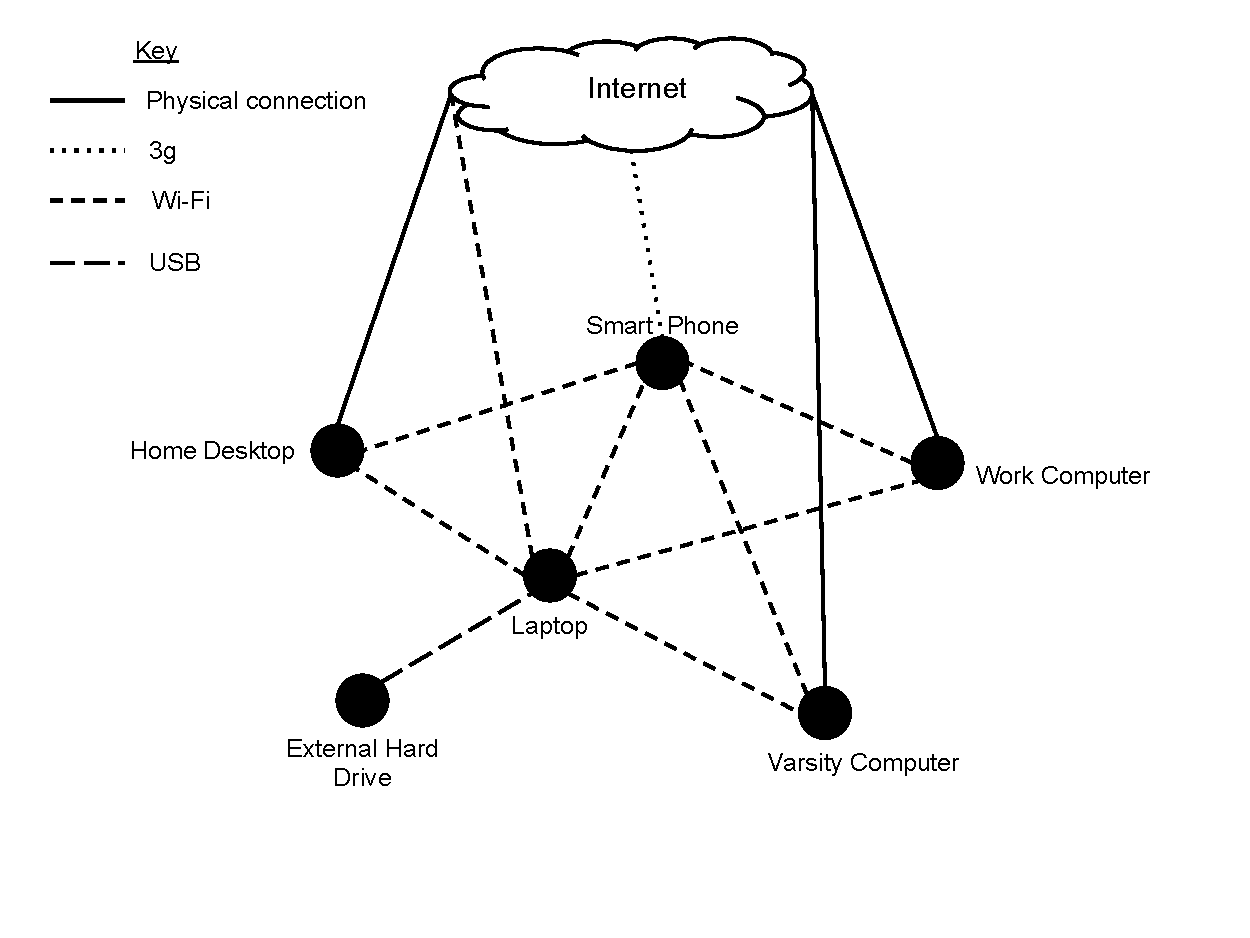
\includegraphics[scale=0.60]{images/PersonalGraph.pdf}
        \caption{Personal Network}
        \label{fig:personal_graph}
    \end{subfigure}
    \begin{subfigure}[b]{1\textwidth}
        \centering
        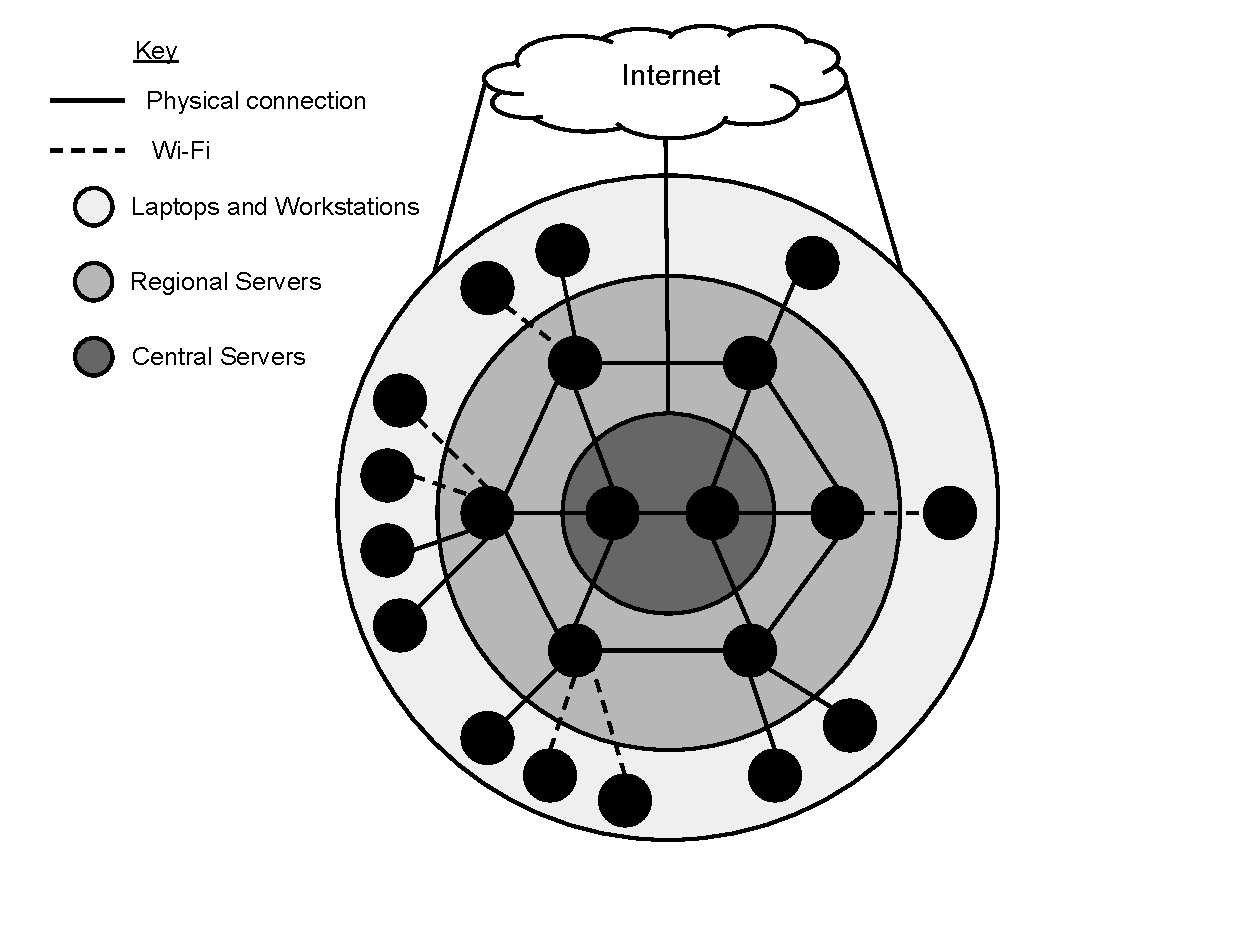
\includegraphics[scale=0.60]{images/CorporateGraph.pdf}
        \caption{Corporate Network}
        \label{fig:corp_graph}
    \end{subfigure}
    \caption{Example use cases}
\end{figure}

The personal network shown in
Figure~\ref{fig:personal_graph} is a graphical representation
of my description above. Figure~\ref{fig:corp_graph}
shows a graph of a corporate network, this
is another example use case. It will have many of the same
basic needs as the personal graph. The coloured rings represent
the need for different policies for different machines in a network.
Unlike Dropbox this is an advantage my system provides.
%Something which Dropbox will not provide but my system does.

% do you need a section to discuss the design of your solution?

%Update this section
\newpage
\section{Architecture and program development}
Before I could begin developing my program, I needed to
have a test environment to run it in. Given that my program
is designed to run across a network of computers I needed
to be able to change links between machines and add or
remove machines automatically for testing purposes.
Doing this manipulation of the network manually would be too time consuming
in the long run. In this section I will discuss how I
control a virtual network of virtual machines for testing, how
I manage the links between them and how I monitor
these links to gather performance statistics regarding the
execution of my program.

\subsection{Virtual machines and node networks}
\label{sec:vm_network}
For testing my program I needed to have a network
of computers that could easily be linked together in different
arrangements. I think of a network of machines as a graph, where
each machine is a node of the graph and the links between machines
are edges in the graph. I decided to use virtual machines for
my network since it means I do not need to have a large number
of physical machines. I can create new machines very easily,
and manipulate the links between them.

I have used Oracle's VirtualBox software. I chose
VirtualBox because of its straight forward command
line interface.
My program should be able to run across
any network of nodes. For this reason I wanted
the potential to be able to test a given arrangement
of nodes.
I decided that I needed to be able change network
topologies easily without having to re-write
my scripts. 

I built some Bash scripts to run on top
of a program called Graphviz.\footnote{www.graphviz.org}
Graphviz is open source software for generating graphical
representations of graphs.
I used Graphviz to generate graphs of all the topologies I worked
with. This made it easy to keep track of what a topology looks like
which was useful for debugging. It was also useful to display results
alongside an image of what the topology looks like. Building my
program on top of Graphviz meant that I could couple the production
of the topology graph and the configuration of the virtual machines.
I never wanted one without the other so this was very useful.

Graphviz takes input from scripts written in DOT language.\footnote{
http://www.graphviz.org/doc/info/lang.html} DOT language is a simple
graph description language.
I have written a script to read in these DOT files and interpret
the graph to set-up my virtual machines (see Appendix~\ref{sec:onTheFly}
 line~\ref{lst:read_dot_file} onwards).
My script also calls a program called Neato (part of Graphviz) to generate 
graphical presentations of graphs.
This means I only have to write one DOT file to get a graph of
my network topology and set-up my virtual machines.
%Graphviz uses a simple notation which made it easy to have
%a Bash script also read this file.

My Bash script enables the appropriate network adaptors on
each virtual machine (see Appendix~\ref{sec:onTheFly} line~\ref{lst:mod_vm_nic}).
It does this by calling the \texttt{VboxManage}, command which provides
a command line interface to VirtualBox's functionality and allows
me to configure the virtual machines to meet my needs.
Then it creates an internal network and attaches these adaptors to use that
network. 
I chose to use an internal network
as the link between any given machines because this way I could
guarantee my program
was the only program using the interface.
This helped me monitor the network traffic generated by
my program (see Section~\ref{sec:iface_mon}).
I sniffed network traffic using packet sniffing tool
Wireshark\footnote{http://www.wireshark.org/}
when my program was not running and also when my program was running
to verify that no other programs were using the interfaces attached to
internal networks.

I started initial tests by writing some simple network topology DOT
scripts. The reason I chose to use simple topologies
when testing my programs was  because it is easier to
visualise how my program runs from the data if the topologies
are simple. The other reason I chose to do this is because
more complex topologies can be thought of as being made up
of many simple topologies. In this way I might be able to
generate a model of how more complicated topologies might
behave by looking at how the program runs in simpler
topologies.
\begin{figure}[htp]
    \begin{subfigure}[b]{0.5\textwidth}
        \centering
        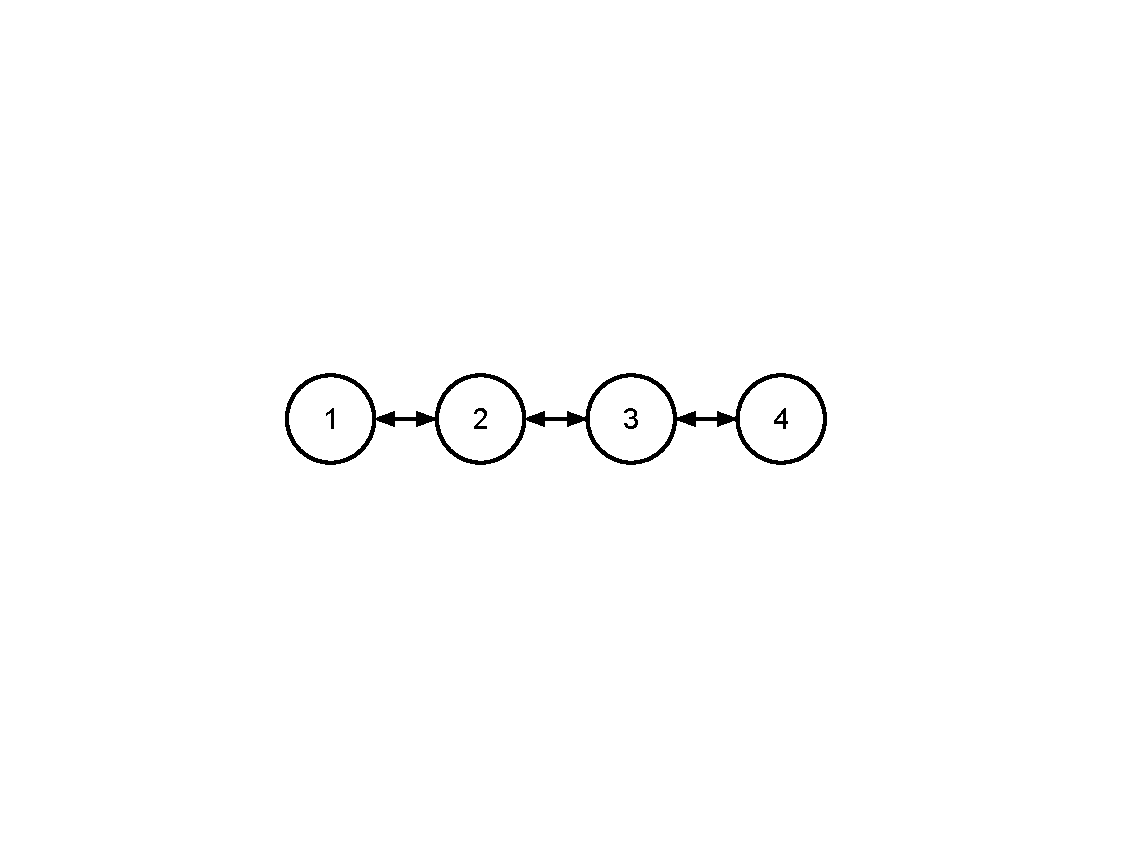
\includegraphics[clip,trim=45mm 60mm 45mm 60mm,width=0.5\textwidth]{images/line-topo.pdf}
        \caption{Line topology}
        \label{fig:line_topology}
    \end{subfigure}
    \begin{subfigure}[b]{0.5\textwidth}
        \centering
        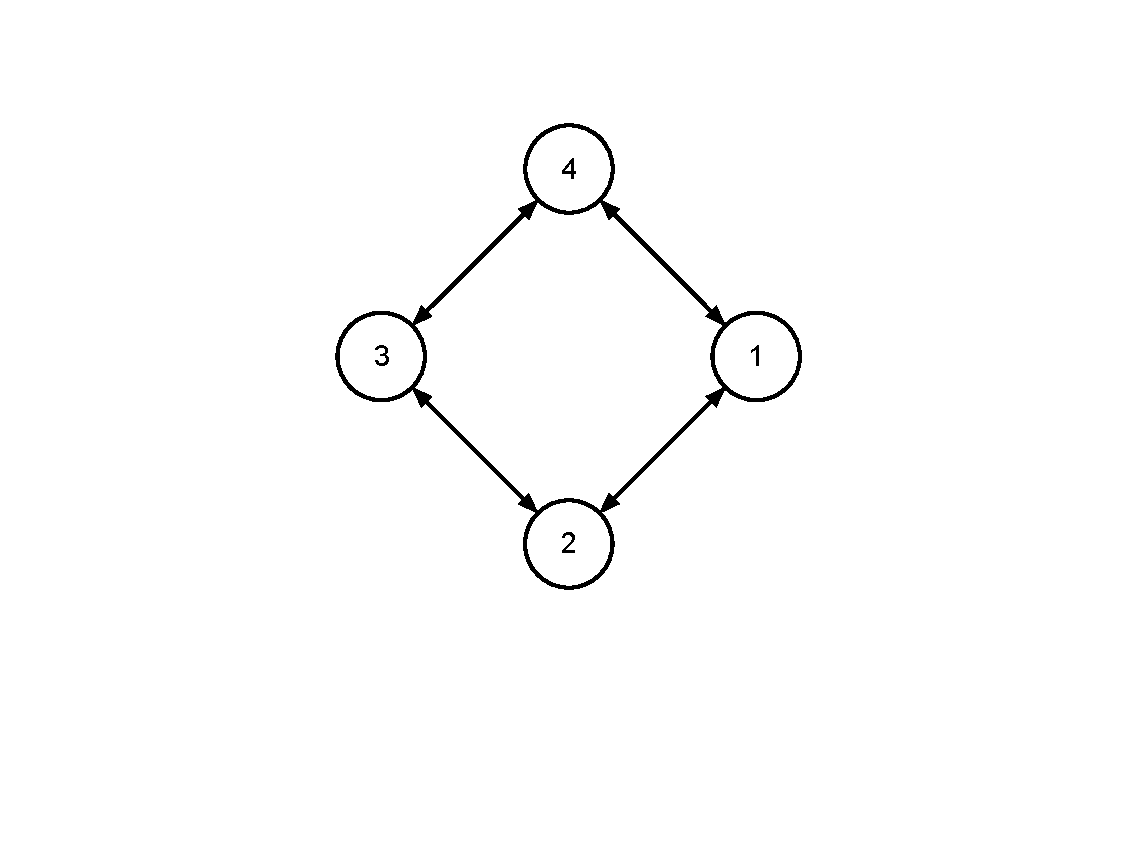
\includegraphics[clip,trim=45mm 40mm 45mm 20mm,width=0.5\textwidth]{images/circle-topo.pdf}
        \caption{Circle topology}
        \label{fig:circle_topology}
    \end{subfigure}

    \begin{subfigure}[b]{0.5\textwidth}
        \centering
        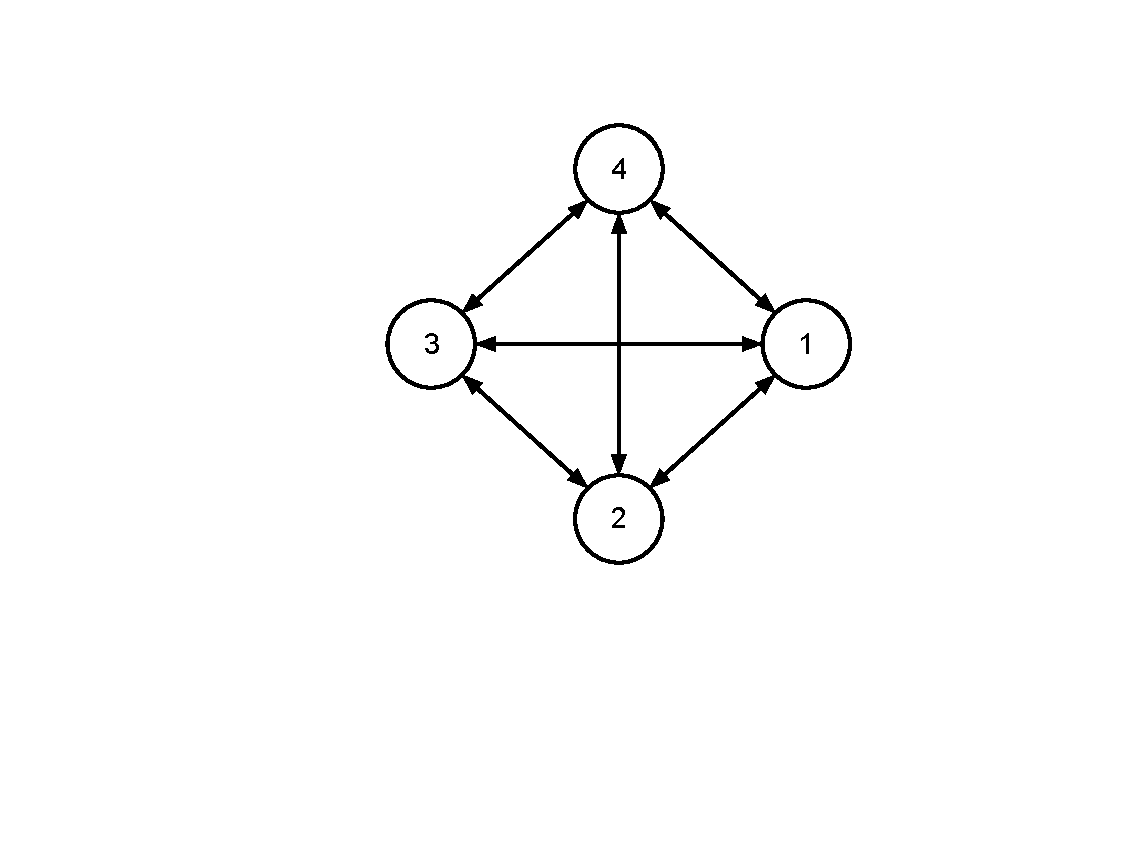
\includegraphics[clip,trim=45mm 45mm 45mm 20mm,width=0.5\textwidth]{images/con-mesh-topo.pdf}
        \caption{Connected mesh topology}
        \label{fig:con_mesh_topology}
    \end{subfigure}
    \begin{subfigure}[b]{0.5\textwidth}
        \centering
        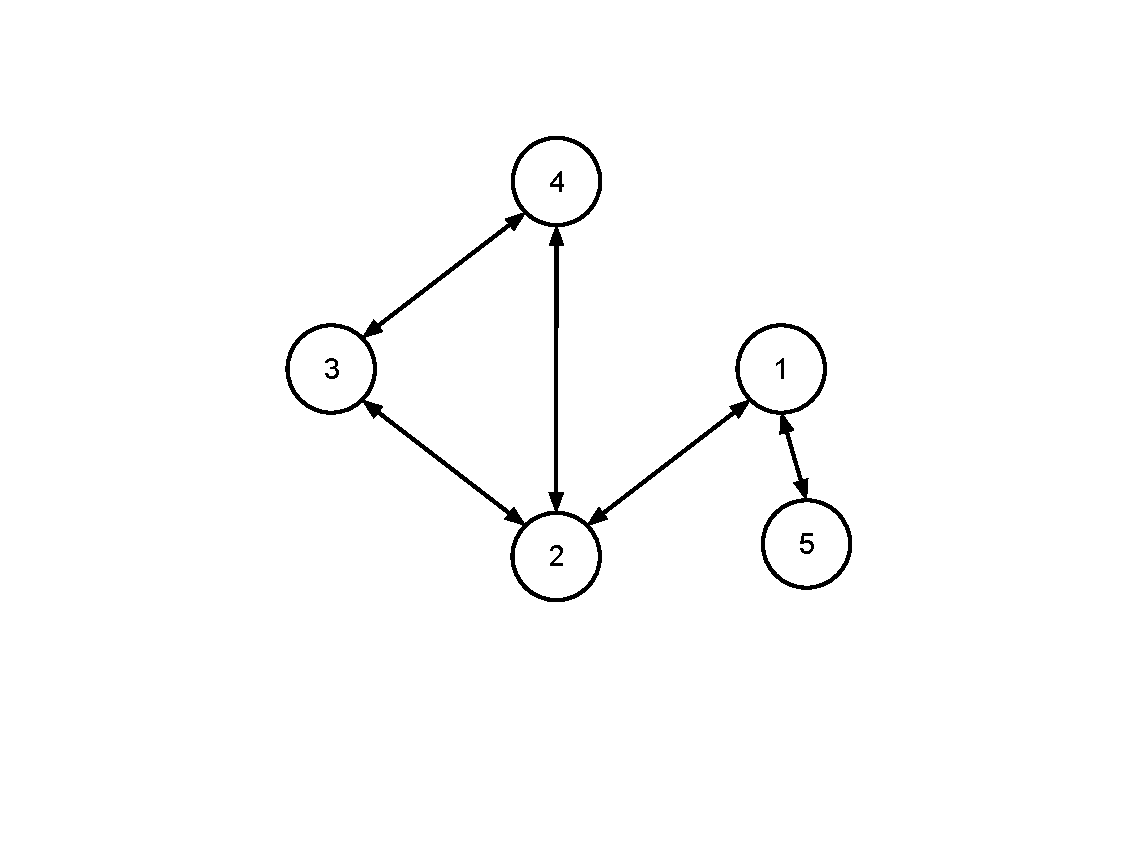
\includegraphics[clip,trim=45mm 40mm 45mm 20mm,width=0.5\textwidth]{images/other-topo.pdf}
        \caption{More complex topology}
        \label{fig:other_topology}
    \end{subfigure}
    \caption{Simple network topologies}
\end{figure}

\begin{comment}
Snippet from one of my network scripts:
\begin{verbatim}
VBoxManage modifyvm "Ubuntu-Test" --nic2 intnet
VBoxManage modifyvm "Ubuntu-Test" --intnet2 "intnet"
VBoxManage startvm "Ubuntu-Test"
\end{verbatim}
\end{comment}

%\newpage

\pagebreak
\subsection{Reading network statistics}
\label{sec:iface_mon}
In order to gather network traffic statistics
I chose to monitor the upload and download
data collected by the interfaces over time.
Given that my program was the only program
using these interfaces I did not have to
differentiate between different processes
using the network.
I looked at the possibility of gathering
statistics on a network where other processes
are using the network connection as you
would expect in a real world application
of my program. For this I found a tool called
NetHogs\footnote{http://nethogs.sourceforge.net/}.
NetHogs runs on Linux and monitors the
amount of data sent over the network by any
given process.
%I also looked at 
%using Iotop\footnote{http://guichaz.free.fr/iotop/}.
%Iotop provides the amount of data being written
%to disk by each process. This was useful because
%the amount of data written relates closely to the amount
%of data sent over the network.
%However I decided that monitoring
%network traffic was a more useful statistic
%as I could also see the \texttt{ssh} overhead
%associated with a transfer.
An interesting challenge I faced when I was trying
to log network usage was what interface to log
data for. Initially I logged the traffic data of all of the
interfaces on the machine (see appendix~\ref{sec:ReadNet}
line~\ref{lst:log_all}). The flaws in this approach
became apparent very quickly; machines with an
internet connection sometimes used large amounts
of data which interfered with the results. It also did not work
with machines that were on more than one internal
network as they might be sending/receiving data
on both of the networks at the same time. I overcame
this problem by using a built-in Linux command \texttt{ip}.
I always had an IP address to send data to, so all
I needed to do was run \texttt{ip route get \{IP address\}}
and examine the route information to see which interface
was being used for communication to that IP 
address (see appendix~\ref{sec:ReadNet} line~\ref{lst:log_ip}).
Once I had the interface name I would then record that
data before and after a sync occurred for that given
interface. I would also do this on the machine I
was sending data to. This would give me timestamps
of when a sync was initiated and when it finished.
Knowing the network traffic statistics before and after
a sync also allowed me to determine how much data each
machine sent or received during a transfer or over
any given time period. I also decided to include
the folder's name being synchronised in the log files.
This was useful for differentiating which sub-node
(See Section \ref{sec:subnodes} for
further details on sub-nodes)
was being synchronised.
%A line starting with
%a \# in my log file denotes a comment. Folder names
%are a specialised version of a comment a \#D indicates
%a folder name. In this way my logging system is robust
%to future changes to my program, I would not have to
%make changes to my scripts which process logs and generate graphs
It would be trivial to add more detailed information to my logs,
such as the IP data is being sent to or received from.
This is a feature I would like to add in the future: I discuss this
possibility further in section~\ref{sec:feedback}.

\newpage
\section{Program design}
In this section I discuss the design decisions I have
made when building my program. This section details
why I chose to use Unison, Python and Inotify to
build a file synchronisation tool. Some of my design
decisions came from running test cases of the program
and reacting to the results I obtained.

%Merge user control and sub-nodes

\begin{comment}
\subsection{settings and stored data}
stores files sync time, how up to date
all graph data could be utilised
\end{comment}

\subsection{Python}
I have chosen to use Python to implement
my program. Python appealed to me because it
supports many different platforms (Windows, Linux, Mac OS~X).
This is useful because it means I will
encounter fewer compatibility problems when running
my program across different operating systems in the future.

\subsection{Unison}
\label{sec:unison}
After looking for cross-platform, open source, file synchronisation
tools, I have found a tool called
Unison\footnote{\url{http://www.cis.upenn.edu/~bcpierce/unison/}}
to be a promising starting
base for this project. Unison is an open source file synchronisation tool.
It supports efficient (\emph{i.e.,} it attempts to only send changes between file versions) file synchronisation between two
directories (including sub-folders) between two ``roots''
that may or may not be on the same machine. Unison calls the
directories it is synchronising, roots.
Section~\ref{sec:point_to_point} looks at how efficient Unison
is at copying files.


%multiproccessing module

\subsection{User control}
One of the main goals of my project is to allow the user
to have a  large amount of control over how the program
behaves. I currently have the program reading from
configuration files that allow the user to specify
which directories they want to watch and where those
directories should be synchronised to.
% give some examples

%I chose to use directories as my granularity for replication
%as opposed to files because keeping track of a large list
%of files may become unwieldy,
% possibly, but you need to be clear what type of unwieldiness you're talking about.
I chose to replicate directories rather than files
because keeping track of a large list of files may become unwieldy.
Because I replicate
directories recursively, I can replicate large amounts
of data without a cluttered configuration file.
Another reason I chose directories as my granularity was because it may be
handy to have a directory full of symlinks pointing to other directories.
% this doesn't necessarily follow: your config file could have the ability to include/exclude files and/or directories (possibly recursively). That would give you expressiveness, and still terse config files for many cases.

%\pagebreak
\subsection{Monitoring directories}
The application needs to monitor directories for changes
(see section~\ref{sec:subnodes})
so that it knows when to perform a sync. The reason I have
chosen to do this is because synchronising a directory that
has not been changed is a waste of time. I do not
however want to be continually polling the watched
directories to see if there have been any changes made.
This would be a significant waste of CPU time and the input/output
time associated with checking the disk. Instead
I have looked into ways of being notified of a
change in the file system below the watched directory.
\begin{itemize}
    \item Inotify
        \begin{itemize}
        \item Inotify is a kernel feature that has been
        included in the Linux kernel since version 2.6.
        It is used to watch directories for changes
        and notify listeners when a change occurs. Inotify
        is inode based and replaced Dnotify, an older system
        that provided the same functionality. Dnotify was
        inefficient, it opened up the file descriptors for
        each directory it was watching which meant the backing
        device could not be unmounted. 
        It also had a poor
        user-space interface which used SIGIO. In contrast Inotify only
        uses one file descriptor and returns events to the
        listener as they occur
        \footnote{www.kernel.org/pub/linux/kernel/people/rml/inotify/README}
        %\cite{inotify-readme}.
        There is a Python module
        called Pyinotify\footnote{http://pyinotify.sourceforge.net/}
        that provides a Python interface
        to Inotify, which I have used in my program.
        Another reason I chose Inotify was because different kinds
        of changes triggered different Inotify events. So I
        can differentiate between a file being deleted, created
        or modified, \emph{etc}.
        \end{itemize}

    \item FSEvents
        \begin{itemize}
        \item FSEvents is an API in 
        MacOS~X\footnote{https://developer.apple.com/library/mac/\#documentation/Darwin/Conceptual/FSEvents\_ProgGuide/Introduction/Introduction.html}
        %\cite{fsevents-intro}.
        It is similar
        to Inotify in that it provides a notification to other
        applications when a directory is changed however
        it does not inform you which file in the directory
        was changed. This does not matter for my
        application since Unison is smart enough not to copy
        unchanged files in a directory. There is a Python module
        for FSEvents called
        MacFSEvents\footnote{http://pypi.python.org/pypi/MacFSEvents/0.2.1}. 
        
        I also looked at using the \texttt{kqueue}
        \footnote{http://developer.apple.com/library/mac/\#documentation/Darwin/Reference/ManPages/man2/kqueue.2.html}
        %\cite{kqueue-man}
        system call that is
        supported by MacOS~X and FreeBSD. It notifies the user
        when a kernel event occurs. However I decided against using
        \texttt{kqueue} as the high level approach of FSEvents
        suits my application's needs.
        \end{itemize}

    %\begin{comment}
    \item ReadDirectoryChangesW
        \begin{itemize}
        \item Windows, like the other operating systems
        I have examined, provides a way of doing this
        too. There is a function called \texttt{ReadDirectoryChangesW}.
% you're not implementing ReaddirectoryChangesW - rephrase?
        There is a FileSystemWatcher Class in .NET version 4 and
        above. IronPython might prove to be a good choice for a
        Windows implementation as it is a version of Python integrated
        with the .NET framework. I have chosen only to implement
        my program on Linux because portability was not in the main
        scope of the project. I would have liked to look
        at it further but it became too time consuming and not interesting
        from a research perspective.
% perhaps clarify why you think it wold be appropriate if you still have more to learn about it.
        \end{itemize}
    %\end{comment}
\end{itemize}

\subsection{Dealing with sub-nodes}
\label{sec:subnodes}
I chose to classify directories as `sub nodes' of a graph. 
The reason I choose directories was because I thought it
would be easier for a user to maintain the configuration file.
A configuration file listing every file to be synchronised could
become very cluttered.
%The reason I choose
%directories is because they are easy to manage a configuration
%file of directories to
%keep in sync (from the users point of view).
If a user wanted to synchronize
certain files in a directory they could write a Unison configuration file with 
exclusions/inclusions in it or use my program's built-in ignore
list (see Section~\ref{sec:uni_and_tmp})
%The other reason directories are a good choice
%is because I can have different directories in different places on different
%file systems by using symbolic links.
I wanted to see how the freshness of different
sub-nodes varied between nodes when the program was running so I tagged
each sub-node when logging information about the programs run 
(see Section~\ref{sec:iface_mon} for more
details on logging). Figure~\ref{fig:line_uni_2dir_comb_graph}
shows a network with two sub-nodes. I alternated between creating
10MB files in each sub-node. The data transferred for the second
sub-node trails the first sub-node in time but a similar amount
of data is transferred over time.

\begin{figure}[htp]
    \centering
    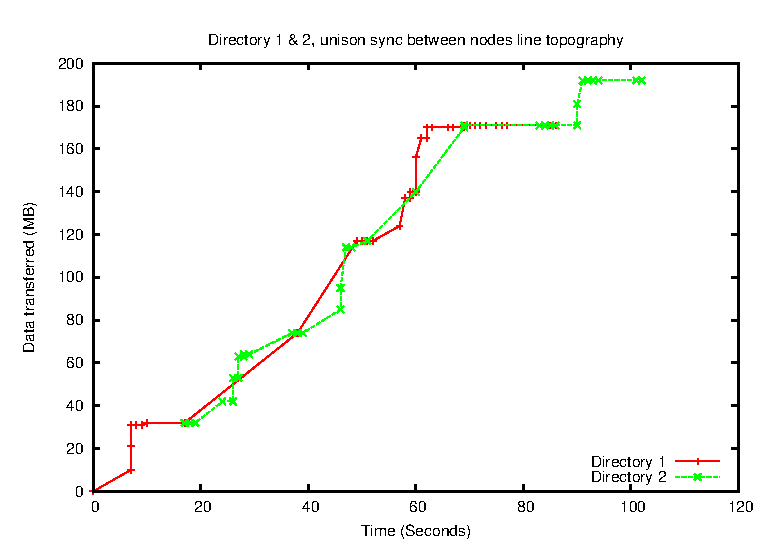
\includegraphics[width=1\textwidth]{images/line-uni-dir-comb.eps}
    \caption{Line topology synchronisation using Unison. Two different directories are being synchronised with 10MB files are sent to each directory alternately every
    ten seconds.}
    \label{fig:line_uni_2dir_comb_graph}
\end{figure}
\newpage

\subsection{Unison and temporary files}
\label{sec:uni_and_tmp}
I noticed that when Unison ran it created temporary files in the
directory and once these files had been fully copied it renamed
them to their intended name. The problem with this was that my program
was picking up these temporary files as they were created and trying to
copy them to the next node, only to find that these files no longer existed.
To get around this problem I decided to implement a filter on the files to
be copied. The program filters out files that contain ".tmp" in the file name.
Unison is not the only program that uses temporary files. I decided that this
should be a user set preference given that users may want to filter out different
files.

My program simply reads from a file with each file name pattern to exclude
listed on a new line. It is easy to add to/remove from. As I said above
I added .tmp to the file as a default. This could easily be extended
to allow a user to omit certain files from the replication by adding
all files in my program's ignore file to Unison's ignore list, or conversely
by maintaining a white list of files to sync. This would allow for
greater granularity when syncing nodes.

\newpage
\section{Program evaluation}
During the development of my program I ran tests after major
changes so that I would know if the program was behaving the
way I expected or not.
When problems arose such as machines continuously polling each
other for changes. I made adjustments to my program to address
these problems.
%In this way I could make changes if
%unforeseen problems occurred.
In this section I discuss
the results from testing my program
and how my results influenced my program.

\subsection{Point-to-Point synchronisation}
\label{sec:point_to_point}
I decided to run some tests using Unison 
and two machines running on the same network to 
determine whether Unison copies data efficiently.

I looked at three methods of file synchronisation across
these two machines. Na\"{\i}ve copying using SCP; using Rsync, an application
designed for efficiently copying files in one direction by looking at
the differences in the files; and Unison as described in Section~\ref{sec:unison}.

\begin{comment}
\begin{figure}[htp]
    \centering
    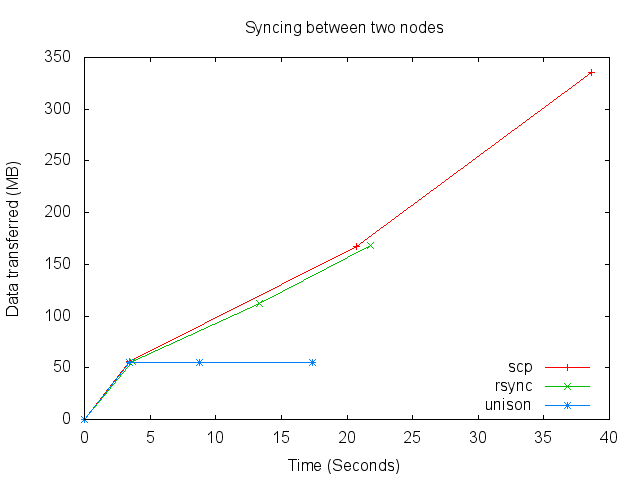
\includegraphics[scale=0.5]{images/two-point-comp-same.png}
    \caption{Comparison of SCP,Rsync,Unison}
    \label{fig:point_comp_graph}
\end{figure}
\end{comment}

\begin{figure}[htp]
    \center{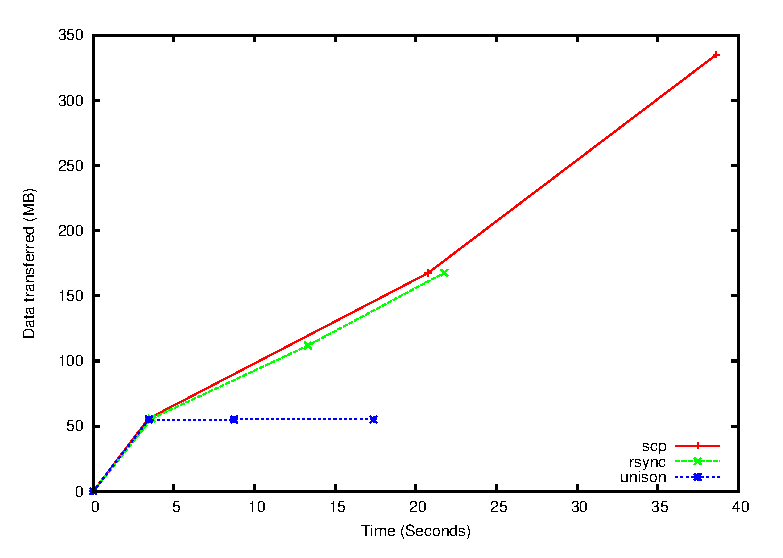
\includegraphics[width=1\linewidth]{images/point-to-point.eps}}
    \caption{Comparison of SCP, Rsync, Unison. Three identical 50MB files 
    with different names are being transfered between two nodes. Each
    point on the graph represents the start or end of a sync.}
    \label{fig:point_comp_graph}
\end{figure}

%Jump right in here with out referencing graph at all, needs to be clearer
%Replace naive copy with SCP since every one knows what SCP is.
Figure~\ref{fig:point_comp_graph} shows how 
Rsync and Unison performed significantly better
than SCP (as expected). After the initial file
transfer, new files added to the directory resulted in much less data
being transmitted over the network, which meant the node graph (see
Section~\ref{sec:vm_network})
became up to date much more quickly.

Figure~\ref{fig:point_comp_graph} shows that SCP sent over 300MB
of data to copy three 50MB
files. This was because SCP is na\"{\i}ve; when it is told to copy a
directory it will copy the entire directory without looking at
the files inside.
This means SCP copies the entire directory each time the directory
is changed. Rsync and
Unison were able to send less data because they work based on the
differences between the files. 
SCP however will copy 50MB after file one is created, 100MB after
the second file is added and finally 150MB when all three
files are present for a total of 300MB.

Rsync copies the expected 150MB for three 50MB files.
Figure~\ref{fig:point_comp_graph} illustrates another advantage
of Unison over Rsync. The graph shows three zero-filled
binary files being copied from one node to the other, one file at
a time. Unison recognised that even though the files were named
differently they had the same content. Another advantage of Unison
is that it handles replication in two directions without
overwriting the files on one node when two nodes have
conflicting changes.

Each of the three methods I trialled had some overhead associated
with them. This overhead was due to the secure shell (SSH) tunnel between
the machines that all three methods used. Unison and Rsync also
incur some overhead when comparing the differences between the files
in the directories. This is why the graph shows the three lines
slightly above where you might expect them to be for the amount
of data that was copied.

\subsection{Full graph replication}
\label{sec:full_graph_rep}
I ran my program on a simple line topology (shown in
Figure~\ref{fig:line_graph}) of all three of my
program's file synchronisation techniques.
Figure~\ref{fig:line_scp} shows SCP performing
poorly compared to Figure~\ref{fig:line_rsync} (Rsync)
and Figure~\ref{fig:line_uni} (Unison). Using Unison and
Rsync each node only received $\approx$30MB, given that
30MB of data was sent to node A this is a pleasing
result. SCP on the other hand sent much more data
than necessary as I have explored in 
Section~\ref{sec:point_to_point}. 


\begin{comment}
\begin{figure}[htp]
    \begin{subfigure}[b]{0.5\linewidth}
        \centering
        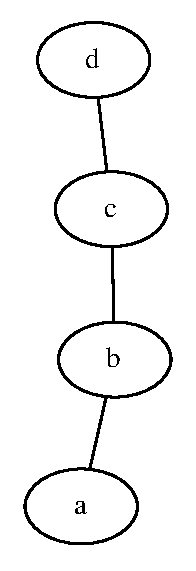
\includegraphics[scale=0.5]{images/line-graph.eps}
        \caption{Line - Generated Graph of Topology}
        \label{fig:line_graph}
    \end{subfigure}
    \begin{subfigure}[b]{0.5\linewidth}
        \centering
        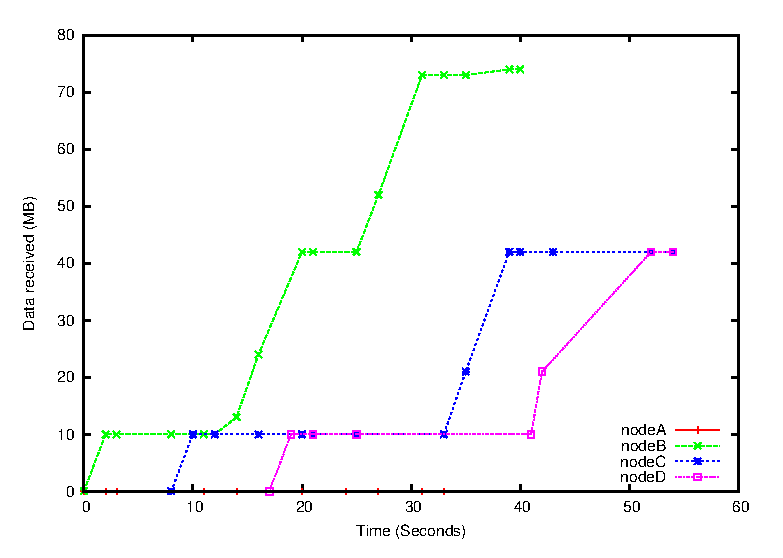
\includegraphics[scale=0.5]{images/line-scp-10-fixes.eps}
        %\center{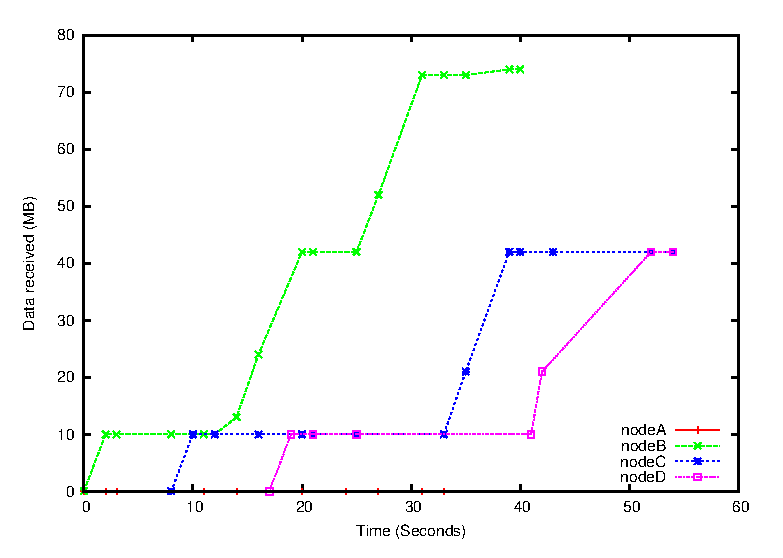
\includegraphics[width=1]{images/line-scp-10-fixes.eps}}
        \caption{SCP}
        \label{fig:line_scp}
    \end{subfigure}

    \begin{subfigure}[b]{0.5\linewidth}
        \centering
        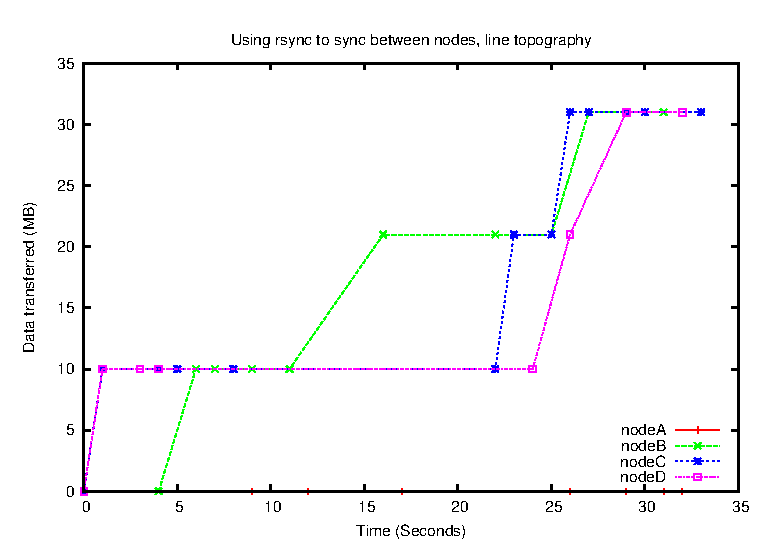
\includegraphics[scale=0.5]{images/line-rsync-10-fixes.eps}
        \caption{Rsync}
        \label{fig:line_rsync}
    \end{subfigure}
    \begin{subfigure}[b]{0.5\linewidth}
        \centering
        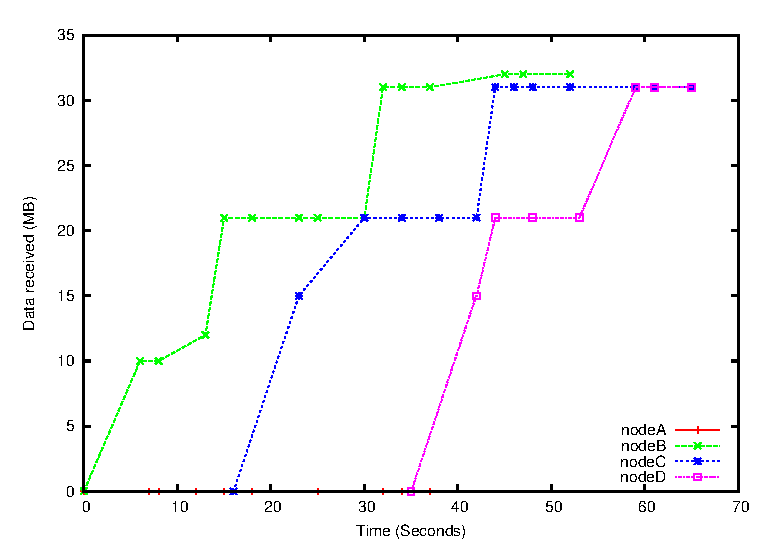
\includegraphics[scale=0.5]{images/line-uni-10-fixes.eps}
        \caption{Unison}
        \label{fig:line_uni}
    \end{subfigure}
    \caption{Comparison of methods over line topology}
\end{figure}
\end{comment}

\pagebreak
\begin{figure}[ht!]
    \centering
    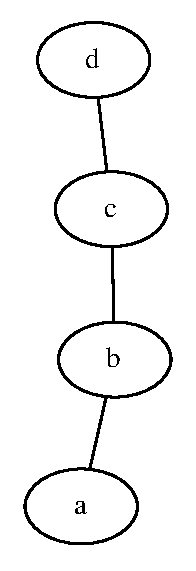
\includegraphics[height=0.4\textheight]{images/line-graph.eps}
    \caption{Generated graph of line topology}
    \label{fig:line_graph}
\end{figure}

\begin{figure}[hb!]
    \centering
    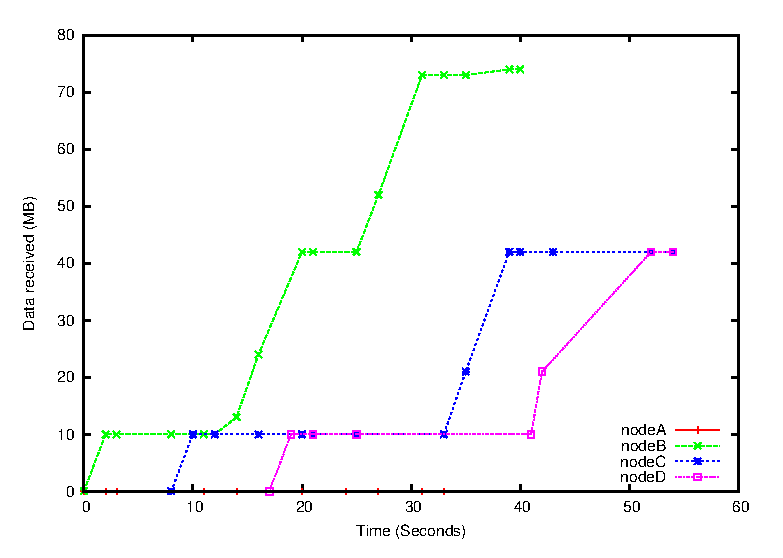
\includegraphics[height=0.4\textheight]{images/line-scp-10-fixes.eps}
    \caption{Program running using SCP. A 10MB file filled with random data
    is being sent every 10 seconds to node A for thirty seconds.}
    \label{fig:line_scp}
\end{figure}

\begin{figure}[ht!]
    \centering
    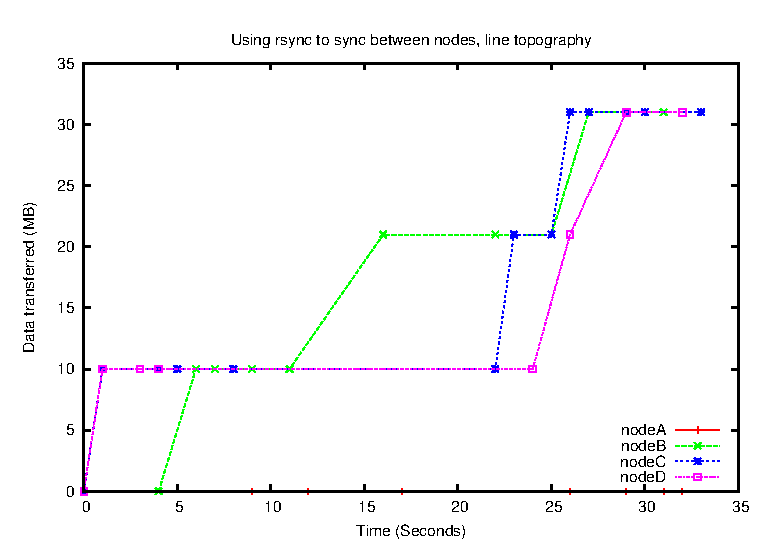
\includegraphics[height=0.4\textheight]{images/line-rsync-10-fixes.eps}
    \caption{Program running using Rsync. A 10MB file filled with random
    data is being sent every 10 seconds to node A for thirty seconds.}
    \label{fig:line_rsync}
\end{figure}

\begin{figure}[hb!]
    \centering
    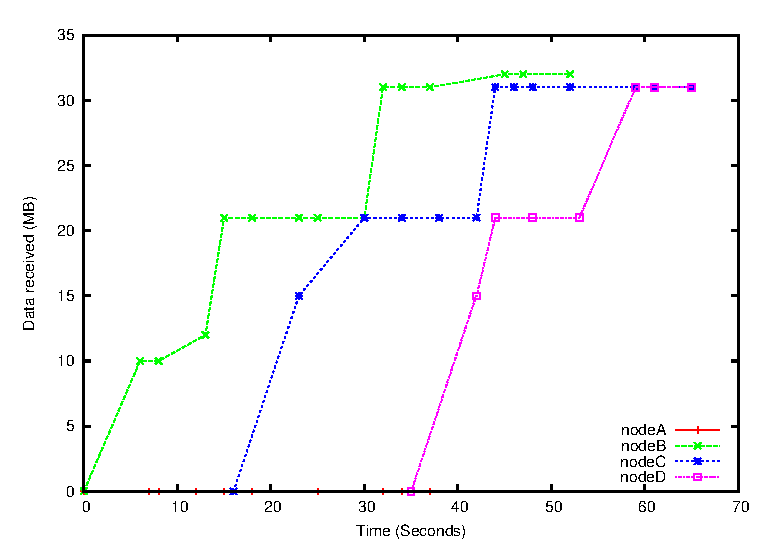
\includegraphics[height=0.4\textheight]{images/line-uni-10-fixes.eps}
    \caption{Program running using Unison. A 10MB file filled with random
    data is being sent every 10 seconds to node A for thirty seconds.}
    \label{fig:line_uni}
\end{figure}
\pagebreak

My program ran smoothly on a line topology so I
set-up some new topologies as shown in 
Figure~\ref{fig:full_circ_graph} and Figure~\ref{fig:full_mesh_graph}.
These were the topology graphs generated by my set-up scripts (see
Section~\ref{sec:vm_network}) I designed them to be a circle
(Figure~\ref{fig:full_circ_graph}), although it does not look like
a circle this is how Neato represented the topology,
and a connected mesh
(Figure~\ref{fig:full_mesh_graph}). 
My program ran as expected with the topologies that
I tested it on. Figure~\ref{fig:full_circ_uni}
shows the results of the circle topology test case.
Figure~\ref{fig:full_mesh_uni} contains the mesh
topology results. These are both graphs of
the program running using Unison. In both cases each node
received $\approx$30MB of data which means each
node received all of the changes created on node A
and that my program successfully replicated data to all
nodes in the network. You can see in Figure~\ref{fig:full_mesh_uni}
that the changes propagated through the graph in a different
order to Figure~\ref{fig:full_circ_uni} this was to be
expected given the more connected nature of the nodes
in the mesh graph.
With the completion of these tests I had achieved
one of my main objectives; to have my program running over
different network topologies.

\begin{comment}
For these tests I stopped using SCP and Rsync as they do
not handle two-way synchronising. If there
are changes coming from two different directions
in the graph one side will potentially overwrite
the other side's changes when using SCP or Rsync.
Rsync does a better job than SCP as it copies the
differences but if there are conflicting changes
one side will be overwritten. Unison on the other
hand will prompt the user for which changes they
want to keep. Given that Rysnc and Unison both
performed similarly in my previous tests up to
this point I decided to continue using just Unison.
\end{comment}

\begin{comment}
\begin{figure}[htp]
    \begin{subfigure}[b]{0.5\linewidth}
        \centering
        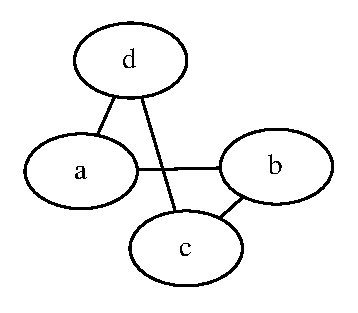
\includegraphics[scale=0.5]{images/circ-graph.eps}
        \caption{Circle - generated graph of topology}
        \label{fig:full_circ_graph}
    \end{subfigure}
    \begin{subfigure}[b]{0.5\linewidth}
        \centering
        %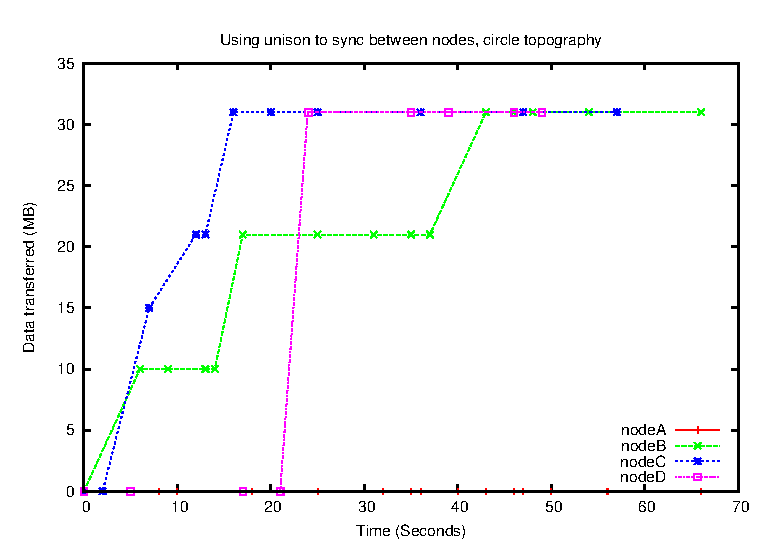
\includegraphics[scale=0.5]{images/circ-uni-10-aite.eps}
        \caption{Unison running over circle topology}
        \label{fig:full_circ_uni}
    \end{subfigure}

    \begin{subfigure}[b]{0.5\linewidth}
        \centering
        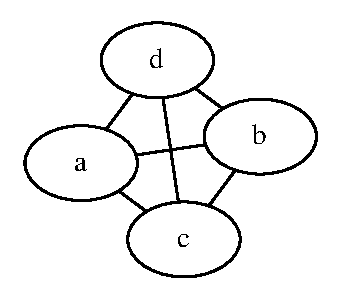
\includegraphics[scale=0.5]{images/mesh-graph.eps}
        \caption{Mesh - generated graph of topology}
        \label{fig:full_mesh_graph}
    \end{subfigure}
    \begin{subfigure}[b]{0.5\linewidth}
        \centering
        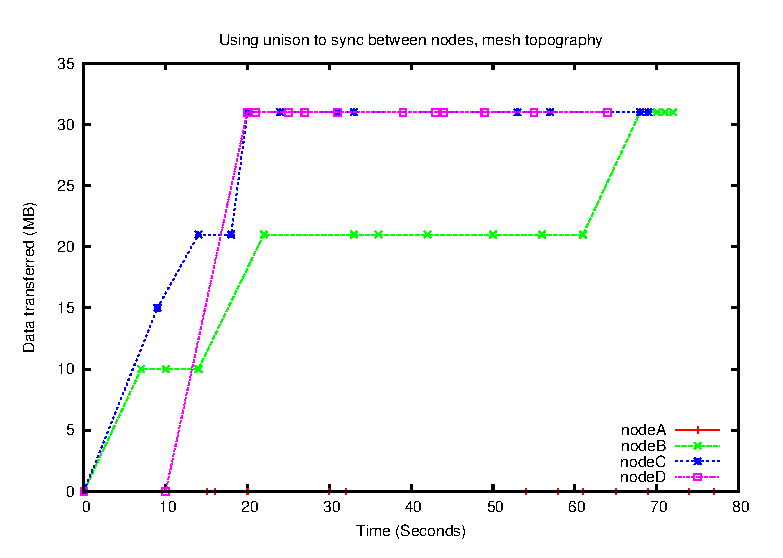
\includegraphics[scale=0.5]{images/mesh-uni-10-aite.eps}
        \caption{Unison running over mesh topology}
        \label{fig:full_mesh_uni}
    \end{subfigure}
    \caption{Comparison of different topologies}
\end{figure}
\end{comment}

\begin{figure}[htp]
    \begin{subfigure}[b]{0.5\linewidth}
        \centering
        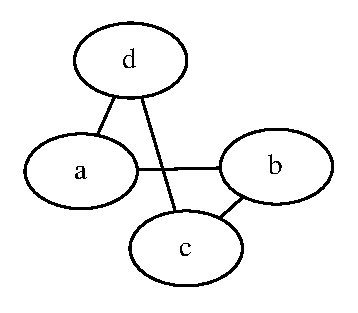
\includegraphics[scale=0.5]{images/circ-graph.eps}
        \caption{Generated graph of circle topology}
        \label{fig:full_circ_graph}
    \end{subfigure}
    \begin{subfigure}[b]{0.5\linewidth}
        \centering
        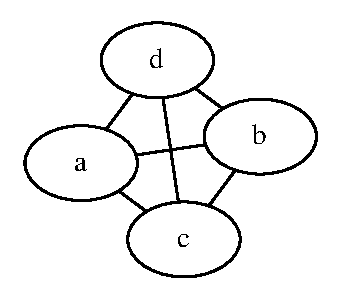
\includegraphics[scale=0.5]{images/mesh-graph.eps}
        \caption{Generated graph of mesh topology}
        \label{fig:full_mesh_graph}
    \end{subfigure}
    \caption{Topology graphs}
\end{figure}

\pagebreak

\begin{figure}[ht!]
    \centering
    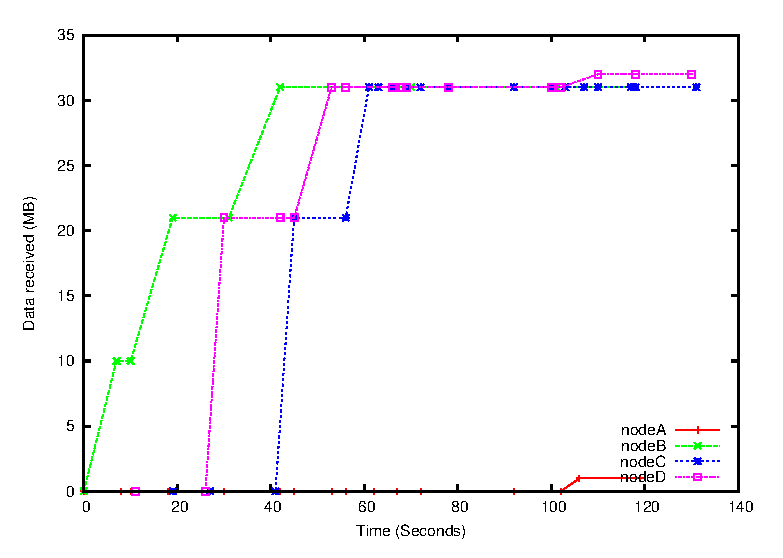
\includegraphics[height=0.4\textheight]{images/circ-uni-almost.eps}
    \caption{My program running using Unison on a circle topology.
    A 10MB file filled with random
    data is being sent every 10 seconds to node A for thirty seconds.}
    \label{fig:full_circ_uni}
\end{figure}
\begin{figure}[hb!]
    \centering
    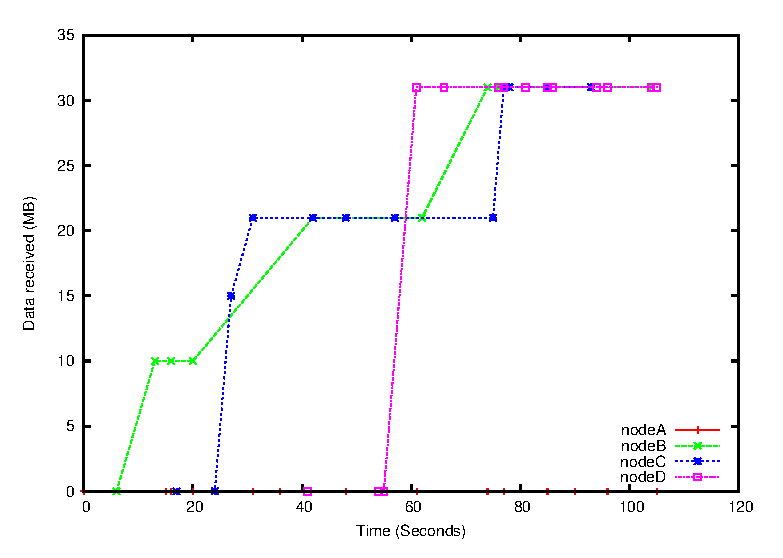
\includegraphics[height=0.4\textheight]{images/mesh-uni-almost.eps}
    \caption{My program running using Unison on a mesh topology.
    A 10MB file filled with random
    data is being sent every 10 seconds to node A for thirty seconds.}
    \label{fig:full_mesh_uni}
\end{figure}

\newpage
\subsection{When to stop copying}
The way my program works is that each node notices when changes
have occurred to a folder it is watching and when a change occurs,
it copies these changes to other nodes specified in the configuration
file.
After testing my program on some simple topologies one problem became
clear; if the changes
came from one of its neighbour nodes the node would notice the change
and send data back to its neighbour this would cause an infinite loop
of two nodes trying to copy changes to each other.
When using Unison this was not as much of
a problem because Unison can detect that no changes had occurred between the nodes
and would stop synchronising after one check (which had minimal overhead). However
for SCP this was a big issue.

\begin{figure}[htp]
    %\centering
    %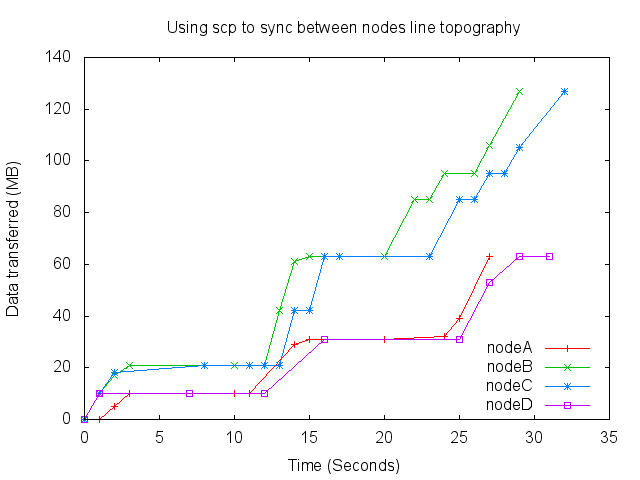
\includegraphics[scale=0.5]{images/line-scp-back.png}
    \center{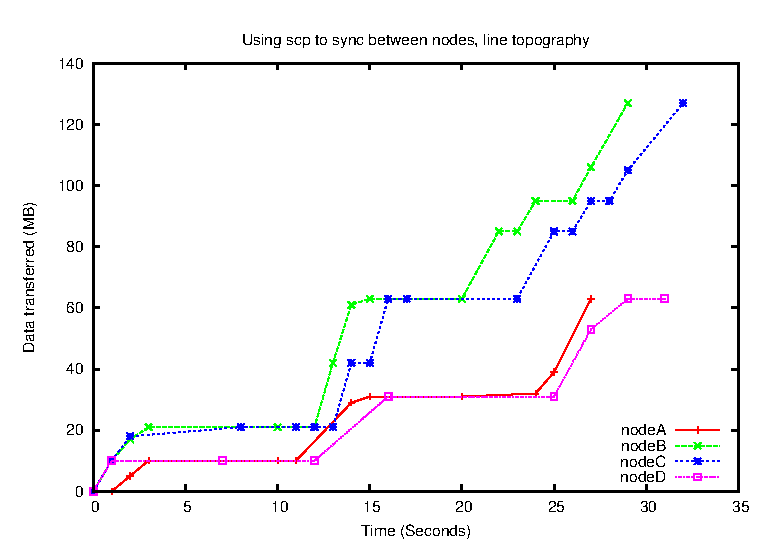
\includegraphics[width=1\linewidth]{images/line-scp-back.eps}}
    \caption{My program using SCP running on a line topology.
    10MB files are being sent every ten seconds to node A. 
    All of the nodes receive more data than they should
    because they are constantly propagating changes to their
    neighbours.}
    \label{fig:line_scp_back_forth_graph}
\end{figure}

Figure~\ref{fig:line_scp_back_forth_graph} shows each node receives
more data than it should. Node B and node C receive over 120MB worth of
data even though there was only 30MB worth of changes and node A
receives over 60MB even though it was the source
of the file changes. My program would have run forever if I had not
stopped it.

%The problem is that node B and node C continue to send
%data to each other even after every node has all of the files. NodeA receives
%a lot of data even though it was the source of the file changes. 

\begin{figure}[ht!]
    %\centering
    %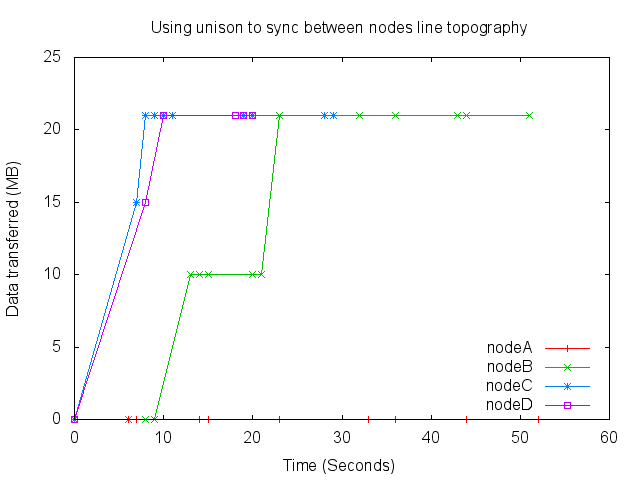
\includegraphics[scale=0.5]{images/line-uni-10-tail.png}
    \center{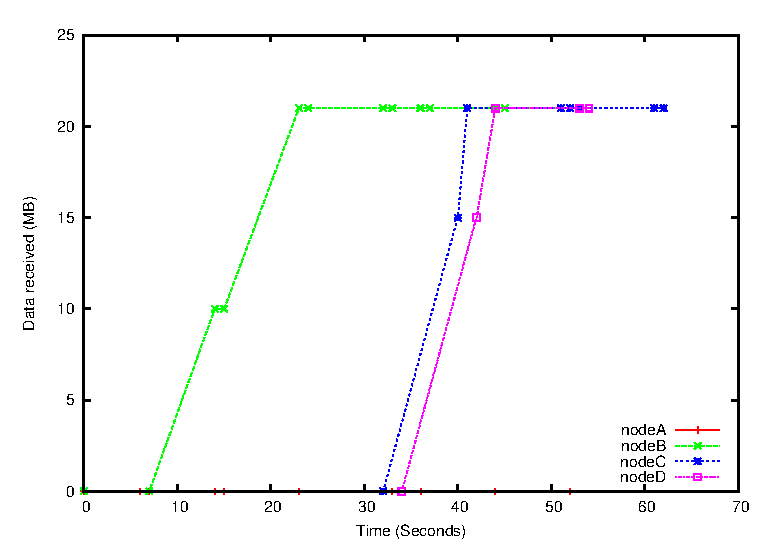
\includegraphics[width=1\linewidth]{images/line-uni-10-tail.eps}}
    \caption{Line topology, using Unison, program continues to check
    for differences in files even after all nodes are the same.
    Each point represents an attempted sync.}
    \label{fig:line_uni_tail_graph}
\end{figure}

The data points in Figure~\ref{fig:line_uni_tail_graph} show that when using
Unison, although no extra data was sent, Unison still had to make checks to see
whether there were any changes or not.

%Change this
To fix this problem I used a control file. Each time a node
synchronised with another node it would write out a control file telling
the other node what files had been copied, who sent them and what the
modification times of the files were. In this way a node could check
if it was about to synchronise a file back to the node it had just received
the file from, or if local changes really had occurred to that file
that were newer than a received file it should continue with its sync.

\pagebreak
\subsection{How often to sync}
So how often should I sync once I notice a change?
If lots of small changes are occurring frequently it might be more efficient
to perform a synchronisation after several changes have occurred. Given that
there is overhead with each synchronisation, fewer copies means less data
sent over the network.

\begin{comment}
\begin{figure}[htp]
    \begin{subfigure}[b]{0.5\linewidth}
        \centering
        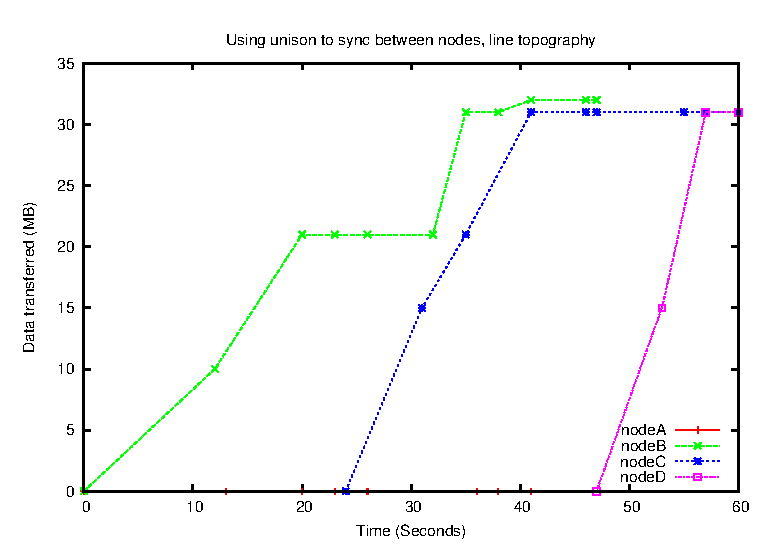
\includegraphics[scale=0.5]{images/line-uni-10-5.eps}
        \caption{5 second sync}
        \label{fig:line_uni_10_5}
    \end{subfigure}
    \begin{subfigure}[b]{0.5\linewidth}
        \centering
        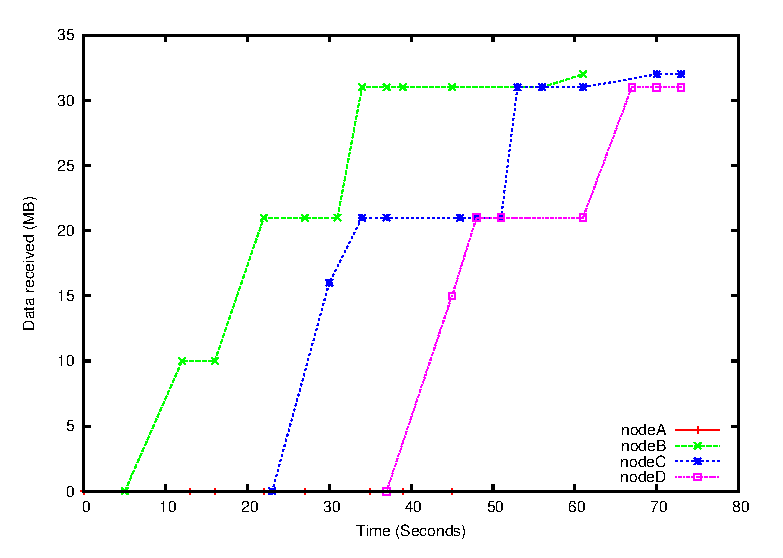
\includegraphics[scale=0.5]{images/line-uni-10-10.eps}
        \caption{10 second sync}
        \label{fig:line_uni_10_10}
    \end{subfigure}

    \begin{subfigure}[b]{0.5\linewidth}
        \centering
        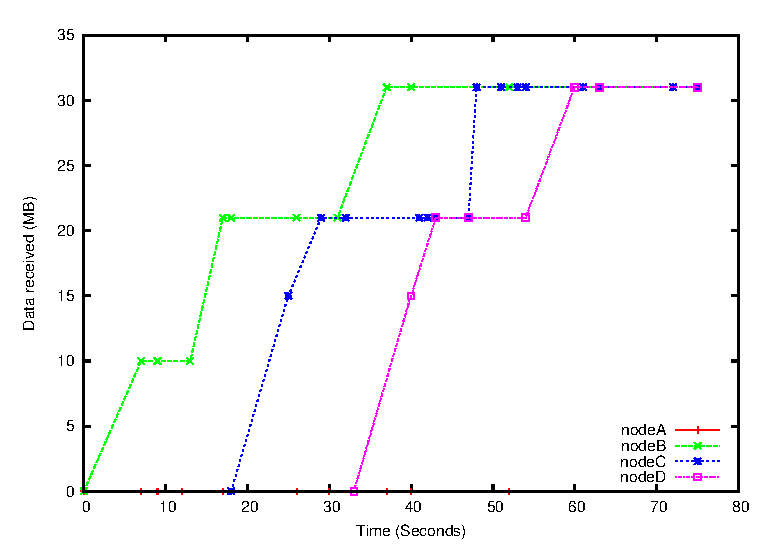
\includegraphics[scale=0.5]{images/line-uni-10-20.eps}
        \caption{20 second sync}
        \label{fig:line_uni_10_20}
    \end{subfigure}
    \begin{subfigure}[b]{0.5\linewidth}
        \centering
        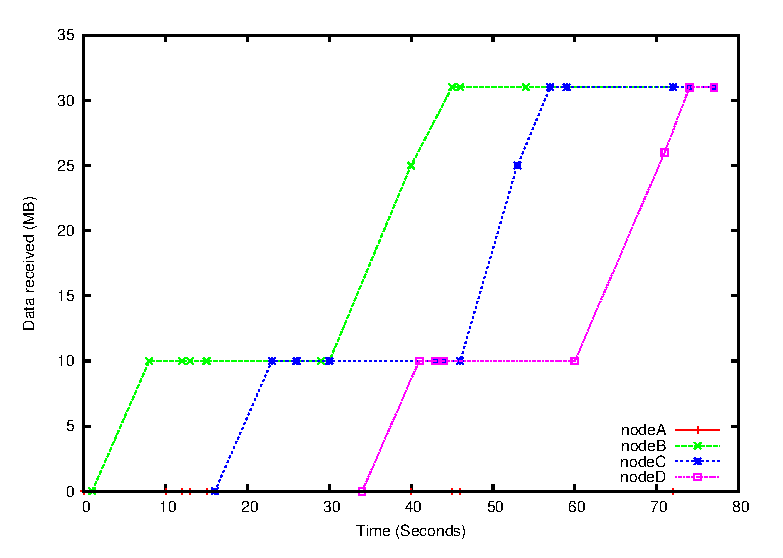
\includegraphics[scale=0.5]{images/line-uni-10-30.eps}
        \caption{30 seconds sync}
        \label{fig:line_uni_10_30}
    \end{subfigure}
    \caption{Comparison how frequently to sync}
\end{figure}
\end{comment}

Figures~\ref{fig:line_uni_10_5},
\ref{fig:line_uni_10_10}, \ref{fig:line_uni_10_20},
and~\ref{fig:line_uni_10_30} show my program running
using Unison to sync 10MB over a network arranged in
a line topology. The files were moved into the watched
directory in ten second intervals. You can see that there is not much
difference between the graphs except Figure~\ref{fig:line_uni_10_5} 
where the time taken for all of the nodes to become up to date
is shorter than the others. In the case of Unison it
is best just to sync as often as possible because Unison
only sends file differences. The only saving when sending
multiple changes at a time is on the SSH overhead
and the overhead associated with Unison comparing the
files. This overhead is negligible when the files
are of any meaningful size.

Figures~\ref{fig:line_scp_10_5},
\ref{fig:line_scp_10_10}, \ref{fig:line_scp_10_20},
and~\ref{fig:line_scp_10_30} show the same 10MB files
being transferred every 10 seconds over the same line topology
as previously
mentioned except I used the SCP option on my program for
these tests.
Figure~\ref{fig:line_scp_10_20} shows that
(20 second delay) the time taken for all nodes to get
the changes was less than
in Figure~\ref{fig:line_scp_10_30} (30 second delay)
%to replicate the
%data from the initial node (A) to the last node (D) in
%the graph. 
%TODO
You can also notice that when the delay was
set to less than or equal to the time the files were
being created (10 seconds) that my program behaved 
in an erratic fashion with some nodes receiving less data
than others. This could indicate an error in my program
or that the data simply takes an odd way through
the graph as it is being replicated as soon as possible.
The data is still replicated in full to each node in the
graph however.
You can see that in Figure~\ref{fig:line_scp_10_11}
that the graph became more uniform as
soon as I increased the delay to 11 seconds.

These results reinforced my idea that the delay should
be set through a configuration file since
the appropriate delay will vary based on how often
the files change. This is currently the case with my
program, users can set a different (or the same)
delay for each folder that they are watching. I
also allow the user to use the `*' wild card character
to tell the program to sync as often as possible. Based
on my findings I would recommend to any user that
%TODO
%This bit is worded unclearly
%the delay be set to more than the frequency that the files
%are changing but not too high as that slows down
%the system. 
the delay time be greater than the average time between
modification of the files but as short as possible as
long delay times slow down replication proportional
to the delay time.
If the user is using Unison they should
set the delay time to be `*' (sync as often as possible)
unless they are trying to synchronise very small files.
%that the delay value be greater than the time the files
%are changed

%TODO: Captions aren't right the need to say what the figure shows
\newpage
\begin{figure}[ht!]
\centering
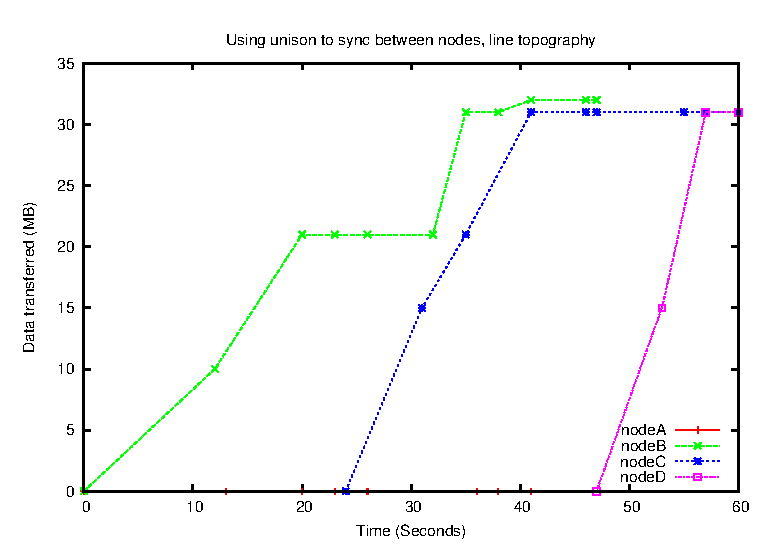
\includegraphics[height=0.38\textheight]{images/line-uni-10-5.eps}
\caption{My program running on a line topology using Unison.
The delay to synchronise time is set to five seconds.
10MB files are being sent every ten seconds to node A. The graph
shows the amount of data received by each node.}
\label{fig:line_uni_10_5}
\end{figure}

\begin{figure}[hb!]
\centering
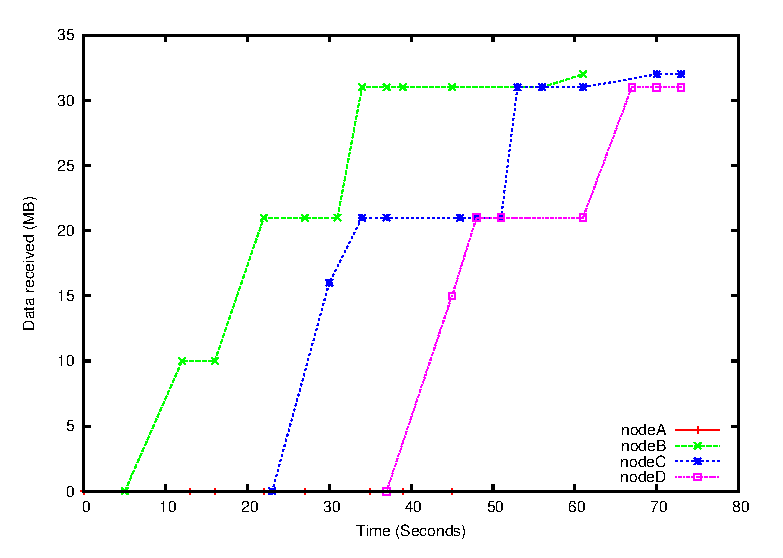
\includegraphics[height=0.38\textheight]{images/line-uni-10-10.eps}
\caption{My program running on a line topology using Unison.
The delay to synchronise time is set to ten seconds.
10MB files are being sent every ten seconds to node A. The graph
shows the amount of data received by each node.}
\label{fig:line_uni_10_10}
\end{figure}

\newpage
\begin{figure}[ht!]
\centering
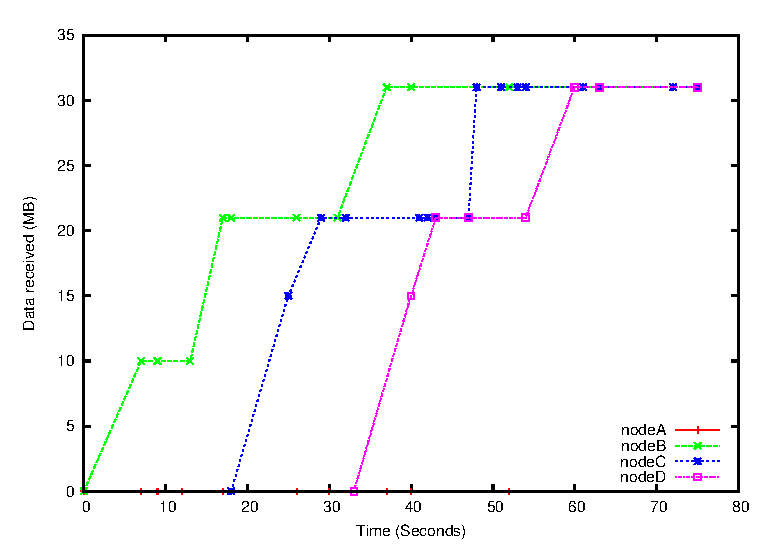
\includegraphics[height=0.38\textheight]{images/line-uni-10-20.eps}
\caption{My program running on a line topology using Unison.
The delay to synchronise time is set to twenty seconds.
10MB files are being sent every ten seconds to node A. The graph
shows the amount of data received by each node.}
\label{fig:line_uni_10_20}
\end{figure}

\begin{figure}[hb!]
\centering
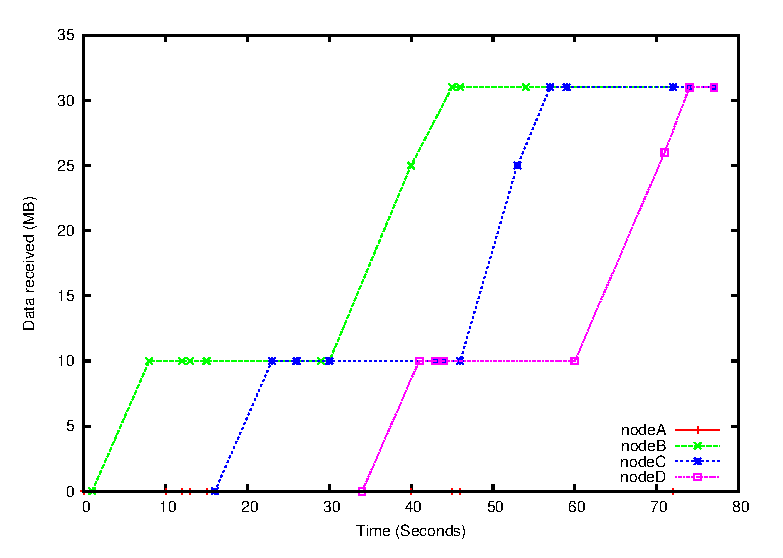
\includegraphics[height=0.38\textheight]{images/line-uni-10-30.eps}
\caption{My program running on a line topology using Unison.
The delay to synchronise time is set to thirty seconds.
10MB files are being sent every ten seconds to node A. The graph
shows the amount of data received by each node.}
\label{fig:line_uni_10_30}
\end{figure}
\newpage

\begin{figure}[ht!]
\centering
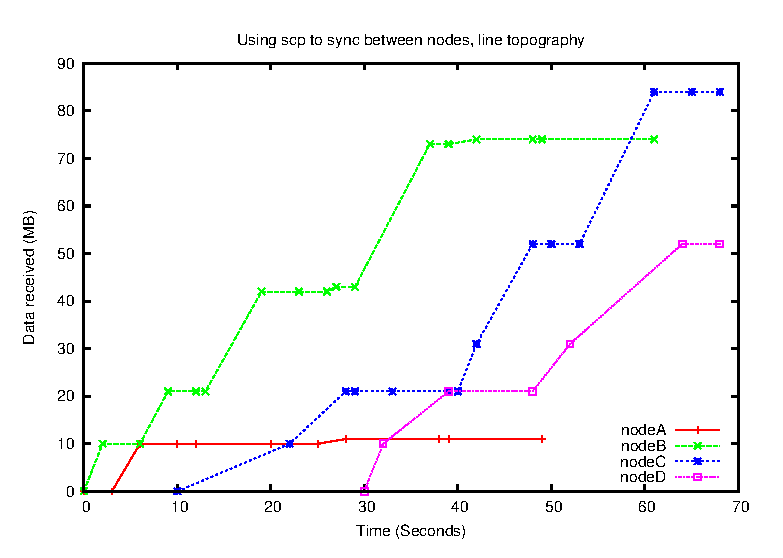
\includegraphics[height=0.38\textheight]{images/line-scp-10-5.eps}
\caption{My program running on a line topology using SCP.
The delay to synchronise time is set to five seconds.
10MB files are being sent every ten seconds to node A. The graph
shows the amount of data received by each node.}
\label{fig:line_scp_10_5}
\end{figure}

\begin{figure}[hb!]
\centering
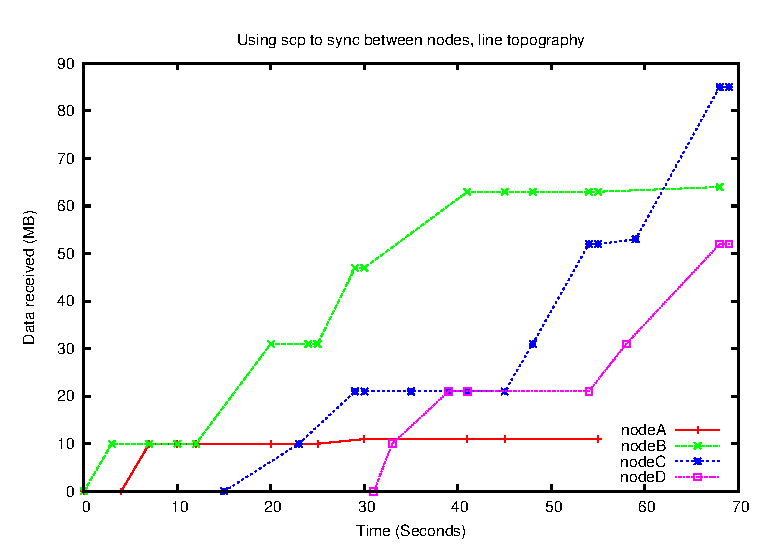
\includegraphics[height=0.38\textheight]{images/line-scp-10-10.eps}
\caption{My program running on a line topology using SCP.
The delay to synchronise time is set to ten seconds.
10MB files are being sent every ten seconds to node A. The graph
shows the amount of data received by each node.}
\label{fig:line_scp_10_10}
\end{figure}

\newpage
\begin{figure}[ht!]
\centering
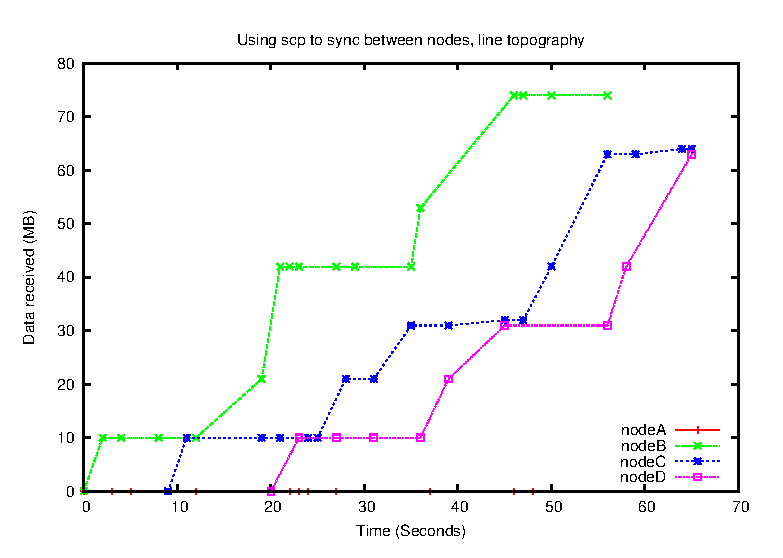
\includegraphics[height=0.38\textheight]{images/line-scp-10-11.eps}
\caption{My program running on a line topology using SCP.
The delay to synchronise time is set to eleven seconds.
10MB files are being sent every ten seconds to node A. The graph
shows the amount of data received by each node.}
\label{fig:line_scp_10_11}
\end{figure}


\begin{figure}[hb!]
\centering
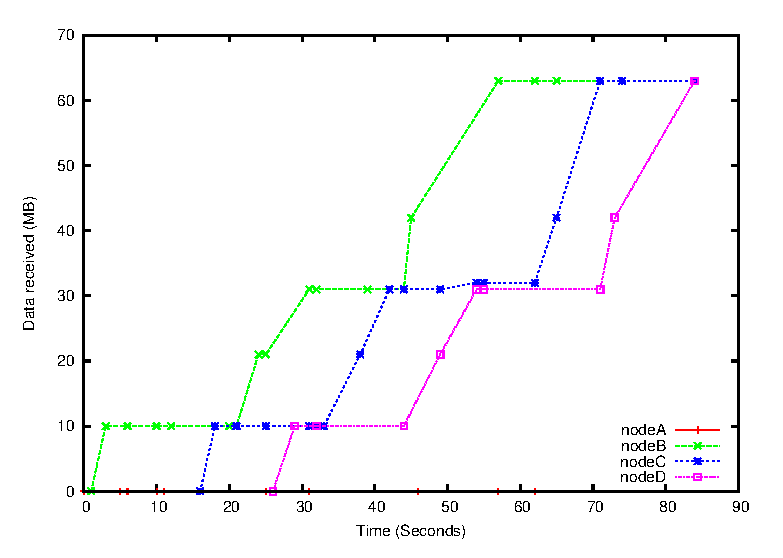
\includegraphics[height=0.38\textheight]{images/line-scp-10-20.eps}
\caption{My program running on a line topology using SCP.
The delay to synchronise time is set to twenty seconds.
10MB files are being sent every ten seconds to node A. The graph
shows the amount of data received by each node.}
\label{fig:line_scp_10_20}
\end{figure}
\newpage

\begin{figure}[ht!]
\centering
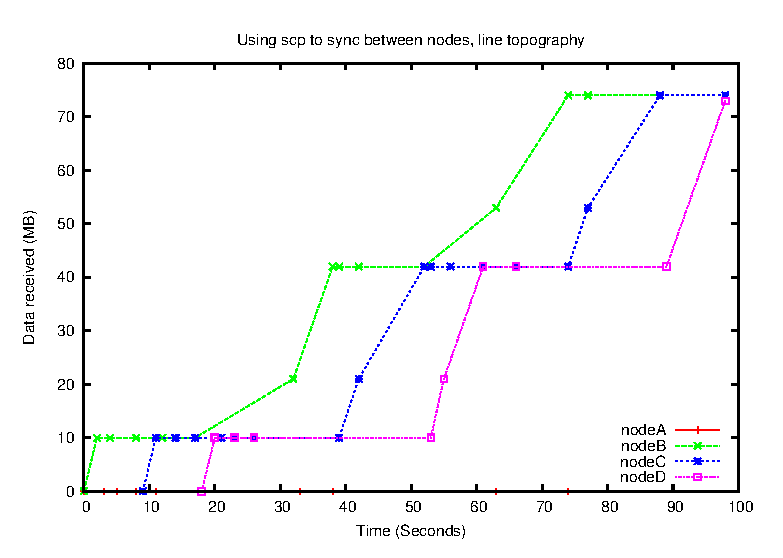
\includegraphics[height=0.38\textheight]{images/line-scp-10-30.eps}
\caption{My program running on a line topology using SCP.
The delay to synchronise time is set to thirty seconds.
10MB files are being sent every ten seconds to node A. The graph
shows the amount of data received by each node.}
\label{fig:line_scp_10_30}
\end{figure}
\newpage

\begin{comment}
\begin{figure}[htp]
    \centering
    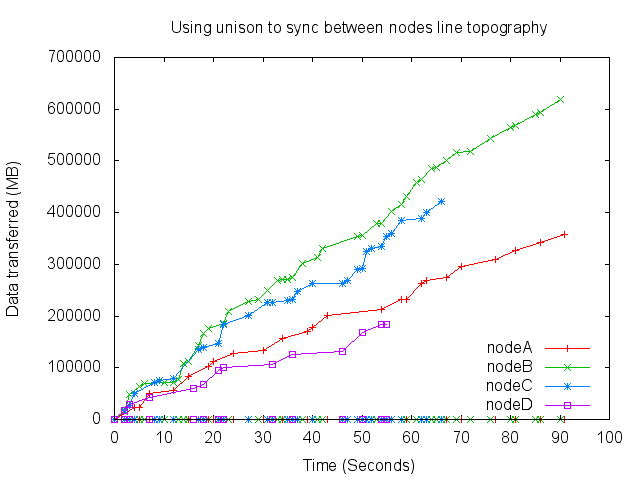
\includegraphics[scale=0.5]{images/rand-txt-2sleep.png}
    \caption{2 seconds sleep text file}
    \label{fig:2sleep_graph}
\end{figure}

\begin{figure}[htp]
    \centering
    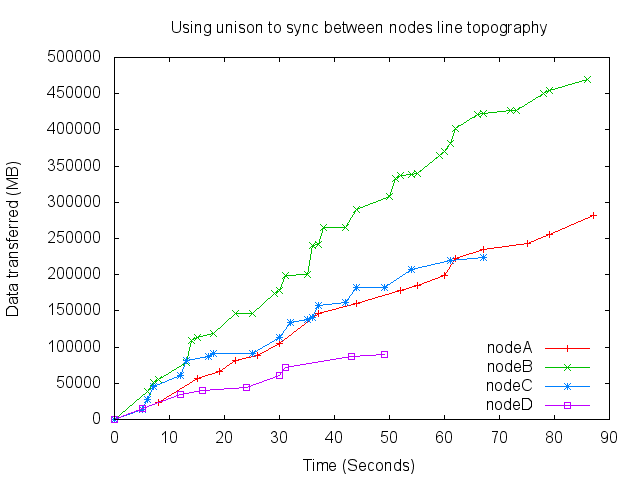
\includegraphics[scale=0.5]{images/5sleep-bad.png}
    \caption{5 seconds sleep text file}
    \label{fig:5sleep_graph}
\end{figure}
\newpage
\end{comment}

\subsection{Wi-Fi vs 3G}
An important use case of my program was where one machine was connected
by a link that a user would not want to use very
often. For example a node might be connected by a 3G link which is slow
and expensive to use. I wanted to make sure that my program could be set to prefer
some links to others. For example to use Wi-Fi whenever possible and try not to
use 3G. I designated the link between node A and node B as a 3G link
in my circle topology (see Figure~\ref{fig:full_circ_graph} in Section~\ref{sec:full_graph_rep}). Node A is linked directly to node B by a slow link and indirectly
by fast links (Wi-Fi link to node D, node D links to node C and node C links
to node B all designated as Wi-Fi links). Previously in Figure~\ref{fig:full_circ_uni} (Section~\ref{sec:full_graph_rep}) node A sent data to
node B and D which then propagated to node C.
In Figure~\ref{fig:circ_uni_thread_100} node B receives data last only after nodes D and C have got the changes.
This is because I set the delay time to 100 seconds between node A and node B
as if it were a 3G link that we do not want to use very often. All the other
nodes had delay times of 10 seconds on their links. My program
spawns multiple threads for each link when a change has occurred in a
watched directory (see Appendix~\ref{sec:WatchAndSync} line~\ref{lst:spawn_thread}).
The thread for the 3G link then sleeps for 100 seconds
and when it wakes looks at the control files of the remote machine to
see that it already has the changes node A was going to send so it aborts.
Node B has already got the files because they travelled through the graph
in the other direction and reached node B before A was ready to send.

\begin{figure}[hb!]
    \centering
    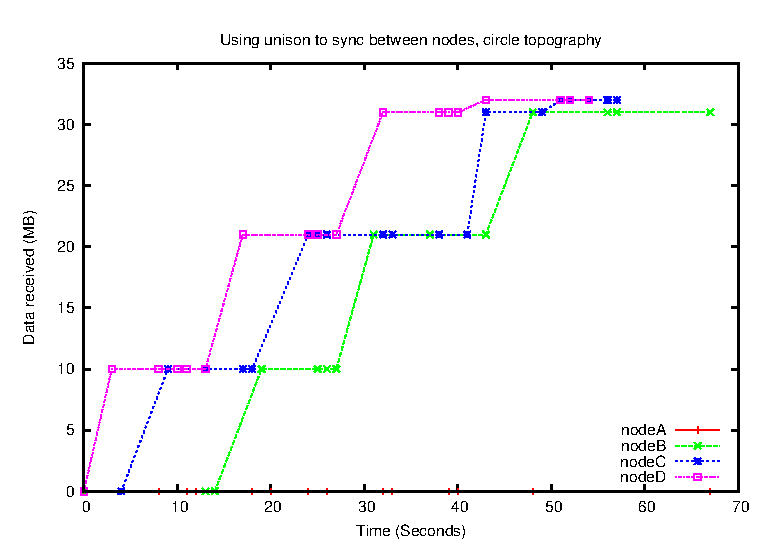
\includegraphics[height=0.4\textheight]{images/circ-uni-thread-100.eps}
    \caption{Node A is connected to node B by 3G, the other links are all Wi-Fi. Three 10MB files are sent to node A over ten second intervals. Node A has a longer delay on sending over 3G than Wi-Fi and node B is the last node to receive the changes.}
    \label{fig:circ_uni_thread_100}
\end{figure}

\newpage
\section{Future Work}
My project ended up requiring a lot of initial set-up
time getting the testing infrastructure ready to
produce different networks and graphs without requiring
user input. As such this drew time away from other
areas of research that I had originally planned to
investigate. The main two areas that I would liked
to have spent more time looking at were mobile nodes
and user/system feedback of data.
When nodes leave and join the graph \emph{i.e.}\ when
nodes leave a network and then join a new network, or
rejoin the old one I call this a mobile node.
I would also have been interested
in seeing how I could have improved the performance
of the program using the statistics the program
gathers as it runs.
%Empty sentence at the end this part needs to be re-written

\subsection{Mobile nodes}
\label{sec:mobile}
Connections between nodes in the graph (edges) may
change over time. This could be because one of the nodes
is a laptop and joins different networks at different
times or because a network/machine is unreliable and is
not up at a given point in time. I have represented
edges that behave in this way as grey on the diagram below.
I will refer to nodes with grey edges as `mobile' nodes.

It would have been interesting to see how mobile nodes affect how
up to date the nodes in the graph are. I predict that
nodes that are not available for very long periods would lag behind
others that are available. I wanted to see what would be
the most effective way of getting these mobile nodes
up to date quickly. Giving mobile nodes priority over
normal nodes might be one solution.
I expect that if a mobile
node is a link between two parts of the network that
these two parts will fall out of synchronisation when the node
leaves the graph. I wanted to look
at how nodes in the graph may 
rely less on unreliable edges. I would like my program
to associate a cost with each edge and prioritise edges
with lower costs when synchronising data. Another option
would be to preference reliable edges and only fall back to using
unreliable edges when necessary. Classifying edges could be
done by cost or by how often an edge is available.

\begin{figure}[hb!]
    \centering
    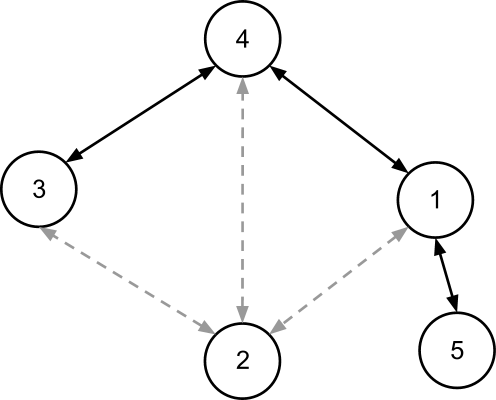
\includegraphics[height=0.2\textheight]{images/mobile-node.png}
    \caption{Node two intermittently has a connection to a subset
    of nodes 1, 3 and 4. The edges in grey are links that are not
    always present.}
    \label{fig:mobile_node}
\end{figure}

\pagebreak

\subsection{Feedback}
\label{sec:feedback}
My program currently keeps detailed logs of the
system state. Logs are kept of the amount of data
transferred between the machines; which files were updated
and when; and the last time the data being watched was updated
by another client (see Section~\ref{sec:iface_mon} for more details
on logging).
I currently have scripts to generate graphs of the data used
and the time taken for the graph to become up to date.
I would have liked to integrate these scripts into my program
to show an end user a graphical representation of the
program running. Integrating my current graph scripts
should be easy since these scripts are written in python
and so is my main program. What would have been very interesting
to look at would be to see if I could use data gathered
from previous runs of the program to see if my program
could estimate future performance based on changes
made to the settings file (like how often to sync a
given sub-node). I envisaged each of the clients
sharing their data with each other to get a view
of the network as a whole and then looking at nodes
that were out of date as candidates for a shorter
sync delay time \emph{etc.} In hindsight I think that this
would have been quite an undertaking, requiring
significant time to develop and should not have
been in the scope of this project.

\newpage
\section{Conclusion}
In this dissertation I discussed the need for a private file
synchronisation tool. I outlined the faults with
current synchronisation tools such as Dropbox. My program
aims to address these shortcomings. I detailed the
implementation details of my program and the design
decisions I made. I showed how I changed my design
when I came across issues.
I tested my program in as many different situations that
I thought would be useful. I have shown that my program
performs better than na\"{\i}ve copying,
works in a variety of situations and behaves in general
how I expect it too.
I achieved my goals of creating a decentralised
file synchronisation tool that will run across any network configuration.
My program allows for fine-grained user control
of settings such as which files should be replicated and how
often they should be synchronised. My program generates
logs of data transferred and the files being synchronised.
This did not lead to detailed statistics about how
the program behaved or heuristics on future behaviour
as I intended. However I was able to generate
graphs from my log files and this could be extended in
a future implementation of my program. Once the user
has written their configuration files the program
operates autonomously as intended. My program has
been a success and does its job of replicating
files well.

%\section{Results}

\begin{comment}
\begin{thebibliography}{9}

%\bibitem{dotcom-trial}
%Foreman, Michael "Kim Dotcom v United States of America". Computerworld. 3 February 2012.

\bibitem{inotify-readme}
www.kernel.org/pub/linux/kernel/people/rml/inotify/README, 22 September 2004.

\bibitem{fsevents-intro}
Apple Inc. \url{https://developer.apple.com/library/mac/#documentation/Darwin/Conceptual/FSEvents_ProgGuide/Introduction/Introduction.html}, 11 October 2011.

\bibitem{kqueue-man}
Apple Inc. \url{http://developer.apple.com/library/mac/#documentation/Darwin/Reference/ManPages/man2/kqueue.2.html}

\end{thebibliography}
\end{comment}

\begin{comment}
\section{Bibliography}
%OPTIONAL: further reading

\section{Glossary}
%OPTIONAL

\section{Index}
%OPTIONAL
\end{comment}

%\section{Appendices}

\newpage

%OPTIONAL
\appendix

\begin{comment}
\begin{figure}[htp]
    \centering
    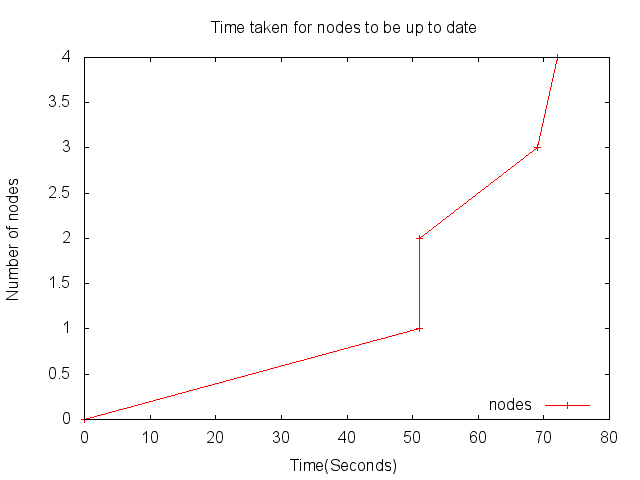
\includegraphics[scale=0.5]{images/fintime.png}
    \caption{Unison, line, finishing times}
    \label{fig:fintime_graph}
\end{figure}
\end{comment}

\lstset{escapeinside={(*@}{@*)}}

\newpage
\section{Program listings}
\subsection{WatchAndSync.py}
\label{sec:WatchAndSync}
\lstinputlisting[numbers=left,language=python,breaklines=true]{code/watchandsync.py}

\pagebreak
\subsection{ReadNet.py}
\label{sec:ReadNet}
\lstinputlisting[numbers=left,language=python,breaklines=true]{code/readnet.py}

\pagebreak
\subsection{ManipVMs.sh}
\label{sec:onTheFly}
\lstinputlisting[numbers=left,language=bash,breaklines=true]{code/onTheFly.sh}

\end{document}
